\part{Wirtschaftlich und politisch pr"agende Faktoren des 19.
Jahrhunderts in Deutschland}
\label{prt:wirtsch-pol}

\chapter{Der Industrialisierungsprozeß in England und Deutschland}
\label{chp:indust-d-e}
\index{Industrialisierung}

\begin{aufgabe}
Erarbeiten Sie aus der Quelle die Faktoren und Begründungen für den
Beginn der Industrialisierung! 

Erläutern sie am unterstrichenen Beispiel das Wirken für die
Industrialisierung in Deutschland!

Begründen sie an der Ausgangslage, warum dieser Prozess in Deutschland
nur verzögert einsetzen konnte!
\end{aufgabe}

\section{Die Vorreiterrolle Englands}
\label{sec:vorr-gb}
\index{Großbritannien!wirtschaftlich}
\index{Industrialisierung!Großbritannien}

\begin{figure}
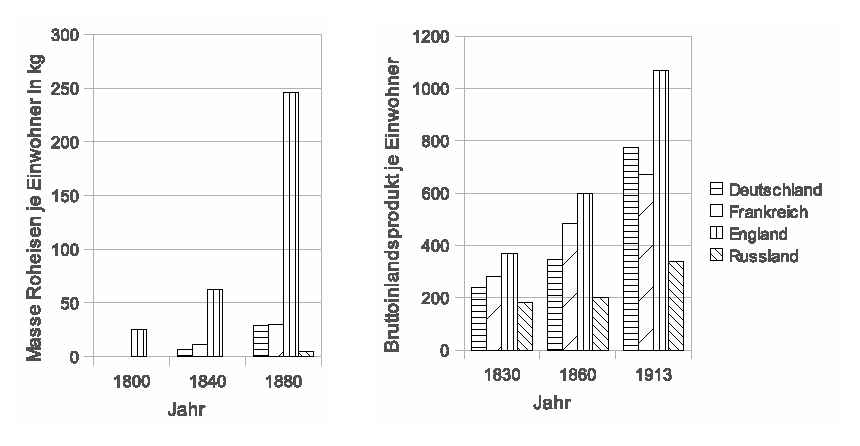
\includegraphics[width=\textwidth]{vorr-gb-diag.eps}
\caption{Roheisenproduktion und Bruttoinlandsprodukt europäischer
Staaten}
\label{pic:vorr-gb-diag}
\end{figure}

\paragraph{Wie Abbildung \ref{pic:vorr-gb-diag} zeigt,} hat
Großbritannien den wirtschaftlichen Entwicklungsprozeß deutlich eher
und mit deutlich höherer Intensität begonnen als andere europäische
Staaten. Es gilt also herauszufinden, wie es zu dieser rasanten
Entwicklung kam.\\

\begin{aufgabe}
Begründen Sie die Vorreiterrolle Englands anhand der besonderen
Voraussetzungen, die dieses Land im Industrialisierungsprozeß
hatte!\footnote{Dazu ist der Inhalt von Abbildung
\ref{pic:vorr-gb-diag} hinreichend}
\end{aufgabe} 

\subsection{Innenpolitische Entwicklung}
\index{Großbritannien!innenpolitisch}

Die \dat{Große Revolution von 1640 bis 1688}
\index{Großbritannien!Große Revolution} \index{Glorious Revolution}
hatte der mittelalterlich"=feudalen Epoche in England ein Ende gesetzt.
Die neue Verfassung sah zensusgebundenes Wahlrecht und
Parlamentssitzvergabe vor und ermöglichte so der \beg{gentry}, den
alten Feudaladel zu verdrängen und ihre fortschrittlichen
wirtschaftlichen Interessen durchzusetzen.

Außerdem sorgte die scharfe Abgrenzung zwischen den Schichten --
Unter-, Oberschicht, Bedienstete etc. -- für eine klare Regelung der
gesellschaftlichen und sozialen Verhältnisse. 


\subsection{Außenpolitische Entwicklung}
\index{Großbritannien!außenpolitisch}

\paragraph{\nam{Henry \Rm{7}} (1486\,--\,1509)} England beginnt eine lange
Tradition der internationalen Seefahrt.

\paragraph{\nam{Elisabeth \Rm{1}} (1558\,--\,1603)} Die englische Flotte
erringt den \dat{Sieg gegen die spanische Armada} und wird so zur
Seemacht. -- Außenhandel und Piraterie weiten sich aus.

\paragraph{\nam{James \Rm{1}} (1603\,--\,1625)} erwirbt 13 Kolonien als
Rohstoffquellen für England und legt so den Grundstein für eine
gezielte Kolonialpolitik.

\paragraph{\Nam{Cromwell, Oliver}{Oliver Cromwell}
(1599\,--\,1658)} England sichert seine Vormachtstellung auf See durch
Siege gegen Holland und Spanien und erwirbt weitere Kolonien, wie zum
Beispiel Jamaika.

\paragraph{\nam{Charles \Rm{2}} (1660\,--\,1685)} Der Krieg gegen
Holland bringt neue Kolonien -- Neuholland und Neuamsterdam.

\paragraph{1714\,--\,1815} Großbritannien erweitert im \dat{War of
Jenkins' Ear 1739\,--\,1742} seinen Kolonialbesitz, erwirbt durch das
Wegfallen Frankreichs als Konkurrenten durch den \dat{Siebenjährigen
Krieg 1756\,--\,1763} Kanada und steigt so endgültig zur Weltmacht
auf.\\

Großbritannien hatte also vor allem durch Handel und Seefahrt einen
gewaltigen Vorrat an Macht, Geld, Rohstoffen, Arbeitern und
Absatzmärkten gewonnen. Dieser bildete die Grundlage für den rasanten
Industrialisierungsprozeß. Abbildung \ref{pic:vorr-gb-gr} bietet
nochmals einen Überblick.

\begin{figure}
\centering
%\begin{sideways}
%\input{vorr-gb-gr.eepic}
%\end{sideways}
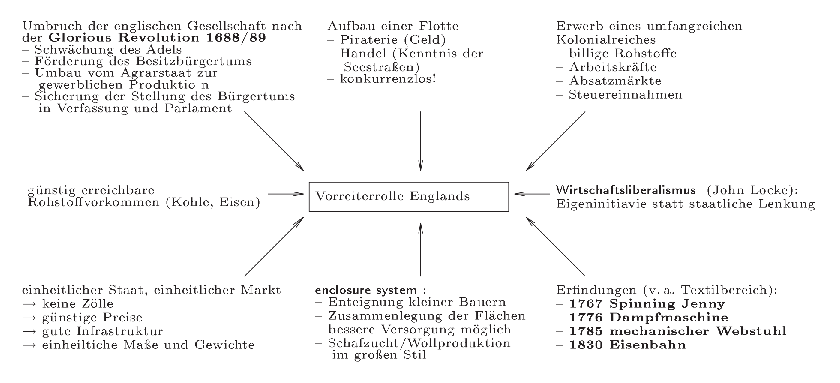
\includegraphics[width=\textwidth]{vorr-gb-gr.eps}
\caption{Ursachen für die Vorreiterrolle Englands}
\label{pic:vorr-gb-gr}
\end{figure}

\endinput

\section{Die Überwindung der Rückständigkeit Deutschlands}
\label{sec:aufh-rueckst-d}
\index{Industrialisierung!Deutschland}

\begin{figure}
\centering
%\begin{sideways}
%\input{vergl-d-e.eepic}
%\end{sideways}
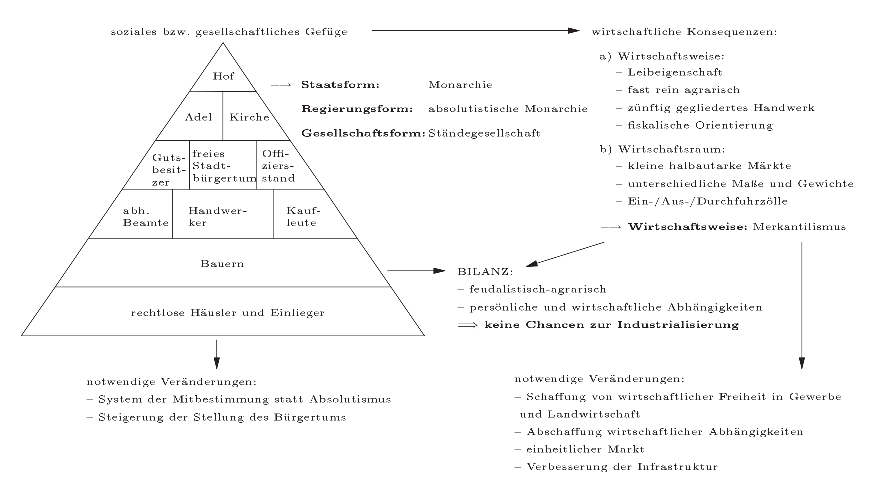
\includegraphics[width=\textwidth]{vergl-d-e.eps}
\caption{Die deutschen Verhältnisse}
\label{pic:dt-verh}
\index{Deutschland!Rückständigkeit}
\end{figure}

\begin{aufgabe}
Zeigen Sie an vier ausgewählten Faktoren, daß Deutschland im
Vergleich zu England als rückständig zu bezeichnen ist!
\end{aufgabe}

\paragraph{Wie Abbildung \ref{pic:dt-verh} zeigt,} waren um 1800
dringend Maßnahmen nötig, um ebenfalls in die industrielle Revolution
einsteigen zu können. Dieser Abschnitt soll zeigen, wie diese
beschaffen waren und was sie bewirkten. \\

\begin{aufgabe}
Stellen Sie an einem Beispiel die Überwindung der Rückständigkeit
Deutschlands im Vergleich zu England dar!
\end{aufgabe}

\subsection[Die Preußischen Reformen]
{Die Preußischen Reformen\footnote{Da die Informationen aus dem im
Geschichtsunterricht gehaltenen Vortrag ungeeignet waren, verwende ich
hier hauptsächlich Material aus \cite{BaswiSchuGesch}.}}
\index{Preußische Reformen}

\mar{Welche Idioten haben damals den Vortrag zu diesem Thema gemacht?}
\begin{aufgabe}
Untersuchen Sie die Preußischen Reformen auf ihre Veränderungen
für das Wirtschaftsgefüge hin!

Fassen Sie sämtliche Informationen zusammen, die zum wirtschaftlichen
Aufschwung Deutschlands als Voraussetzung anzusehen sind und stellen
Sie deren Wirkung dar!
\end{aufgabe}

\paragraph{Nach dem \dat{Krieg gegen Napoleon 1806/1807}} war Preußen
dem Zusammenbruch nahe. Daraufhin initiierten fortschrittliche und
einflußreichende Persönlichkeiten -- allen voran Reichsfreiherr
\Nam{Stein, Karl vom und zum}{Karl vom und zum Stein} und Fürst
\Nam{Hardenberg, Karl August von}{Karl August von Hardenberg} -- eine
Reihe von tiefgreifenden Reformen, die den Wiederaufbau und die
Befreiung des Staates von der französischen Fremdherrschaft
ermöglichen sollten.

Damit einher ging auch eine wirtschaftliche Reform Preußens, dessen
auf dem System der persönlichen Abhängigkeit beruhende Gutswirtschaft
von am Wirtschaftsliberalismus orientierten Grundsätze abgelöst
wurde.

\subsubsection{Bauernbefreiung}
\index{Bauernbefreiung}
\index{Regulierungsedikt}
\index{Oktoberedikt}

Das \dat{Oktoberedikt von 1807} hob die Erbuntertänigkeit und damit
die Leibeigenschaft auf und ermöglichte ihnen den Besitz von eigenem
Land. Die Gutsbesitzer wurden gemäß dem \dat{Regulierungsedikt von
1809} entschädigt.

Der so geschaffene \emph{freie Bauernstand} war nun in den
Wirtschaftsprozeß integriert und also an Produktionssteigerungen
interessiert.

\subsubsection{Städteordnung}
\index{Städteordnung}

Mit der \dat{Einführung der Städteordnung 1808} gewährte Preußen seine
Städten die selbständige Verwaltung ihrer Angelegenheiten. Die Bürger
konnten fortan aktiv und passiv an der an einen niedrigen Zensus
gebundenen Wahl zur Stadtverordnetenversammlung, die
wiederum Magistrat und Bürgermeister (Exekutive) wählte, teil- und
damit auf die Politik Einfluß nehmen.

Dies sind die Ursprünge der kommunalen Selbstverwaltung in Deutschland.

\subsubsection{Verwaltungsreform}
\index{Verwaltungsreform}

Die \emph{Verwaltungsreform} sollte
\textquote[\cite{BaswiSchuGesch}]{einen lestungsfähigen, sparsamen
und bürgernahen Staatsapparat [\dots] schaffen.} Dazu gehörten eine
Vereinfachung der Behördenstruktur durch eindeutige Klärung der
Zuständigkeiten und die Trennung von Justiz und Verwaltung. Möglich
wurde dies durch die neuen Ein"-stel"-lungs- und Laufbahnkriterien für
Beamte (Qualität statt Gunst) und die fortschreitende
Verschriftlichung und Archivierung von Vorgängen. -- Das
Berufsbeamtentum, wie es heute noch fast unverändert in Deutschland
besteht, wurde geprägt. -- Außerdem wurden die Beamten durch relativ
hohe Gehälter bestechungssicher gemacht.\mycite{WikPreusRef}

Ein weiterer bedeutender Inhalt der Verwaltungsreform war die
Schaffung des \emph{klassischen Kabinetts} aus Ministerien (fünf an
der Zahl) mit klar abgegrenzten Ressorts.

\subsubsection{Gewerbereform}
\index{Gewerbereform}

\dat{1810/11 wurde die Gewerbefreiheit} eingeführt. -- Um ein Gewerbe
aufzunehmen genügte der Erwerb eines Gewerbescheins.
\mar{Gewerbe\-steuer? -- Stimmt. Einfügen!} Damit ging die Aufhebung
des Zunftzwangs und somit die Beseitigung zahlreicher Monopole einher.
Dies und die weitgehende Abschaffung der staatlichen Aufsicht über die
Wirtschaft beförderte Konkurrenz und freien Markt.

\subsubsection{Folgen}

\begin{itemize}
\item Unabhängigkeit von den Gutsherren bringt ehemalige Bauern als
Arbeitskräfte in die Städte.
\item zunehmende Bedeutung des Gewerbes auch in ländlichen Gebieten
\item zunehmende Verstädterung
\item später: Verschärfung der sozialen Frage durch übermäßige Zunahme
der Zahl der Handwerker bei starker Konkurrenz
\end{itemize}


%%%%%%%%%%%%%%%%%%%%%%%%%%%%%%%%%%%%%%%%%%%%%%%%%%%%%%%%%%%%%%%%%%%%%%

\subsection{\dat{Die Fr"uhindustrialisierung 1770\,--\,1850}}
\label{ssc:frueh-ind}
\index{Fr"uhindustrialisierung}

\begin{aufgabe}
Stellen Sie Ansätze wirtschaftlichen Aufschwunges in Deutschland
anhand der Frühindustrialisierung dar!

Bewerten Sie die Wirkungsweise dieser auf den
Industrialisierungsprozeß insgesamt!
\end{aufgabe}

\paragraph{Die Verarbeitung von Agrarprodukten} wie sie in
Zuckerfabriken, Branntweinbrennereien, Brauereien, Ölmühlen und
Tabakfabriken betrieben wurde, bildete die Wurzeln des
Unternehmertums. So wurde beispielsweise der Zuckerrübenbauer zum
Zuckerfabrikanten und der Textilverleger zum Textilfabrikanten.

\paragraph{Die Textilproduktion beruhte auf dem Verlagssystem}
(beispielsweise heimgewerbliche Leinenherstellung), das in dieser
Phase der Industrialisierung zur Blüte kam
\mycite[207]{gelbesGeschichts}.  Mit der \dat{Einführung mechanischer
Webstühle 1830} wurden dann die Voraussetzungen für die
Textilindustrie geschaffen.

\paragraph{Ferner erschloß man neue Industriezweige,} wie den
Kohlebergbau und die Erzgewinnung.\\

Diese Ansätze wirtschaftlichen Aufschwungs schufen einen Bedarf nach
Maschinen. -- Kleine Reparaturwerkstätten entwickelten sich zu
Maschinenfabriken. -- Man benötigte Metall. -- Um die isolierten
Produktionsinseln zu verbinden, mußte man die Infrastruktur aufbauen.
-- Man baute 1835 die erste Eisenbahnstrecke. -- Wieder brauchte man
Metall.

Hier zeigen sich die Grundlagen der \beg{Interdependenzen} -- starker
Rückkopplungseffekte, die die folgende rasante Entwicklung
Deutschlands vom Agrar- zum Industriestaat bedingten.

Die Wirtschaft selber entwickelte sich in der Zeit der
Frühindustrialisierung allerdings nur langsam.

%%%%%%%%%%%%%%%%%%%%%%%%%%%%%%%%%%%%%%%%%%%%%%%%%%%%%%%%%%%%%%%%%%%%%%

\subsection{Der Zollverein}
\label{ssc:zollv}
\index{Zollverein}

\begin{aufgabe}
Stellen Sie den Entstehungsprozeß des Zollvereins dar!

Bewerten Sie seine Bedeutung für den Wirtschaftsaufschwung/die
Industrialisierung in Deutschland!
\end{aufgabe}

\subsubsection{Entstehungsprozeß}

\paragraph{Vorläufer:} süddeutscher Zollverein, mitteldeutscher
Handelsverein, preußisch-hessischer Verein

\begin{chronik}
\item[1.\,1.\,1834]
\dat{Zollvereinigungsvertrag} zwischen den Vorläufervereinen -- Der
\emph{deutsche Zollverein} entsteht.

\item[bis 1854]
Westerweiterung durch Anschluß weiterer Länder

\item[1857]
Einführung des Zollvereinstalers

\item[1867]
Norderweiterung

\item[1868]
verbindliche Einführung von \emph{Meter und Kilogramm}
\index{metrisches System}

\item[1871]
Zollverein ist vollständig\footnote{Zur Zusammensetzung des
Zollvereins siehe
\href{http://de.wikipedia.org/wiki/Gebiet_des_Deutschen_Zollvereins}
{diesen Wikipediaartikel}}
\footnote{Österreich wurde trotz Antrages nicht aufgenommen, da das
den Verein dominierende Preußen seine Rivale durch die zusätzlichen
Zahlungen schwächen konnte.}
und umfaßt zur Reichsgründung das gesamte Reichsgebiet
\index{Deutsches Reich}
\end{chronik}


\subsubsection{Politische Bedeutung}

\begin{itemize}
\item ökonomische und materielle Verbindung der Deutschen zu einer
\emph{Nation}
\item Vorbereitung einer echten Nation
\item Stärkung der materiellen Kraft der deutschen Lande durch Wahrung
der auswärtigen Gesamtinteressen
\item Verschmelzung einzelner Provinzialinteressen zu einem
Nationalinteresse -- Erweckung eines Nationalgefühls
\end{itemize}

\subsubsection{Wirtschaftliche Bedeutung}

\begin{itemize}
\item \mar{?} Wiedergeburt des deutschen Unternehmergeistes
\item \mar{?} Teilhabe der deutschen an allen
Nationalangelegenheiten 
\item \mar{?} Anteilnahme des Mittelstandes und der
Großgrundbesitzer an praktischer Politik
\item Grundlage für einheitlichen Markt
\item Wegfall der Zollschranken
\item einheitliche Währung und Maßeinheiten
\end{itemize}

$\Longrightarrow$ Bedingung für ein modernes Wirtschaftssystem


%%%%%%%%%%%%%%%%%%%%%%%%%%%%%%%%%%%%%%%%%%%%%%%%%%%%%%%%%%%%%%%%%%%%%%

\subsection{Der neue Unternehmertypus}
\index{Deutschland!Unternehmertum}

\begin{aufgabe}
Zeigen Sie, daß sich in Deutschland ein neuer Unternehmertypus
Herausbildete und stellen Sie ihn vor!

Begründen Sie, daß er einen Beitrag zur Überwindung der
Rückständigkeit Deutschlands leisten konnte!
\end{aufgabe}

\subsubsection{Entstehung von Unternehmen}

\begin{itemize}
\item Handwerker bauen auf technischen oder finanziellen Grundlagen
oder auf Basis einer Idee Werkstätten zu Fabriken aus.
\item \beg{Feudalunternehmer}
\item Unternehmensgründung auf Basis von Kapitalbesitz oder Erbschaft
(z.\,B. \Nam{Krupp, Alfred}{Alfred Krupp}
\end{itemize}

\subsubsection{Entwicklung zum \emph{neuen} Unternehmer}

Private Unternehmer, Techniker, Kaufleute, Wissenschaftler und
Politiker unternahmen Bildungsreisen nach Großbritannien, von wo sie
Technologien und Anregungen für das deutsche Bildungswesen
mitbrachten. Sie importierten auch britische Maschinen und knüpften
Beziehungen, über welche sie britische Fachleute nach Deutschland
holten.

Hier entwickelte sich eine neue Art, Unternehmen zu gründen: Man
setzte risikofreudig teilweise das gesamte Eigen- oder auch
Familienkapital ein. Wo dieses nicht reichte, schlossen sich mehrere
Unternehmer zusammen -- man gründete Aktiengesellschaften -- oder
wurden Kredite aufgenommen -- Großbanken, wie die \ins{Deutsche Bank}
oder die \ins{Dresdner Bank} entstanden.

\subsubsection{Mitwirkung der Unternehmer bei der Überwindung der
Rückständigkeit Deutschlands}

\begin{description}
\item[Wissen und Erfahrung:] Import von technischen Neuerungen,
Maschinen, Facharbeitern und Ingenieuren
\item[Bildungssystem:] Übergang zu innerdeutscher Ausbildung von
Fachkräften und Ingenieuren an Fachschulen und technischen Hochschulen
\item[Aufschwung des Finanzwesens:] hohe private Investitionen und
damit verbundenes Risiko
\item[technischer Fortschritt:] Kapitalismus führt zu hohem
Konkurrenzdruck -- Unternehmen verbessern eigenständig Produktions-
und Verarbeitungsprozesse. (forschendes Unternehmertum)
\end{description}

Damit war bald sowohl die finanzielle wie auch die technologische
Unabhängigkeit vom Ausland gewährleistet. Die neuen Unternehmer trugen
so maßgeblich zum Aufbau eines wirtschaftlich konkurrenzfähigen
deutschen Kaiserreiches bei.

%%%%%%%%%%%%%%%%%%%%%%%%%%%%%%%%%%%%%%%%%%%%%%%%%%%%%%%%%%%%%%%%%%%%%%

\subsection[Veränderungen in der Infrastruktur]
{Veränderungen in der Infrastruktur \mycite[157/158]{braunesGeschichts}}

\begin{aufgabe}
Weisen Sie nach, daß eine Verbesserung der Infrastruktur in
Deutschland stattgefunden hat!

Bewerten Sie die Bedeutung dessen für den Industrialisierungsprozeß!
\end{aufgabe}

\paragraph{Die Verbesserung der deutschen Infrastruktur} begann in der
Zeit der Frühindustrialisierung: Man befestigte die Landstraßen, baute
Flüsse aus und verband sie durch Kanäle. Dampfschiffe erleichterten
und beschleunigten den den Gütertransport.

\paragraph{Die weitaus bedeutendste Veränderung} war aber die
Einführung der Eisenbahn \index{Eisenbahn} in Deutschland. Nur
sinnvoll durch den Zollverein (\emph{siamesische Zwillinge}) erfuhr
sie seit ihrem \dat{ersten Einsatz 1935} eine rasante
Entwicklung\footnote{Zu konkreten Zahlen siehe
\cite[159]{braunesGeschichts} und \cite{WikEisenbahn}} und wurde zum
entscheidenden Motor der Industrialisierung.

Einerseits erleichterte, beschleunigte und verbilligte sie den
Personen- und Warenverkehr erheblich. Dadurch eröffneten sich nicht
nur neue Möglichkeiten, Rohstoffe zu beschaffen beziehungsweise
Produkte zu vertreiben, sondern förderte ebenso den kulturellen
Austausch und vergrößerte die Anzahl der Arbeiter in Form von
Pendlern.

Andererseits befeuerte die neue riesige Nachfrage nach Stahl für
Schienenverlegung und Eisenbahnherstellung die Schwerindustrie und den
Arbeitsmarkt. Deren Expansion verlangte wiederum nach weiterem Ausbau
der Eisenbahn und so weiter. -- Diese äußerst starke
\beg{Interdependenz} führte in der Folge den sprunghaften Anstieg der
Wirtschaftsmacht Deutschlands.



%%%%%%%%%%%%%%%%%%%%%%%%%%%%%%%%%%%%%%%%%%%%%%%%%%%%%%%%%%%%%%%%%%%%%%

\subsection{Entstehung von Industriegebieten -- Das Ruhrgebiet}
\index{Industriegebiete!Entstehung}
\index{Ruhrgebiet}

\begin{aufgabe}
Zeigen Sie am Beispiel des Ruhrgebietes die schrittweise Entstehung
industrieller Ballungsgebiete!

Bewerten Sie die Bedeutung solcher Ballungsgebiete für den
Industrialisierungsprozeß!
\end{aufgabe}

\subsubsection[Entstehungsprozeß]{Entstehungsprozeß\footnote{Hier am
Beispiel des Ruhrgebiets. -- In anderen Gebieten ähnlich.}}

\begin{enumerate}
\item heranwachsende Stahlindustrie seit 1820 -- Strukturwandel von
Landwirtschaft zu Industrie nach Kohlefunden
\item 1840\,--\,1848 Ausbau von Eisenbahn und Binnenschiffahrt führt
zur Verbesserung der Infrastruktur
\item Übergang vom Stollen- zum Schachtbau
\item Eröffnung von Zechen in großer Zahl führt zu starker Zuwanderung
\item Eisenindustrie ab 1850, forcierte Entwicklung durch Eisenbahnbau
\item 1850\,--\,1870: Kohle!
\item Land- und Intensivwirtschaft zur Versorgung der Bevölkerung in
den Randgebieten der Ballungszentren
\item Nachfolgeindustrien
\end{enumerate}

\subsubsection{Bedeutung der Ballungsgebiete für den
Industrialisierungsprozeß}

\begin{itemize}
\item kein Zoll
\item kürzere Transportwege
\item Zusammenarbeit der Unterhehmen
\item Konzentration von Fachpersonal
\item Konzentration von Wissenschaft und Forschung
\item Investition der Rendite in neue Techniken, Betriebe etc.
\end{itemize}

$\Longrightarrow$ Sprungbrett für die Industrialisierung des gesamten
Landes

\endinput



\chapter{Die \emph{Soziale Frage} und Ansätze für deren Lösung}
\label{chp:soziale-frage}
\index{Soziale Frage}

\begin{aufgabe}
Die Industrielle Revolution wird in der historischen Betrachtung als
Segen und Fluch bezeichnet. Nehmen Sie zu dieser Sichtweise wertend
Stellung! 
\end{aufgabe}

\section{Die Entstehung der Arbeiterschaft als Klasse}
\label{sec:arb-klas-entst}
\index{Arbeiterklasse}

\mar{irgendwie mehr Geographie -- Wo bleiben die Arbeiter?} Ausgehend
von der \dat{Bevölkerungsexplosion ab circa 1800}, deren Ursachen die
Aufhebung der ländlichen Eheverbote, medizinische und
landwirtschaftliche Fortschritte waren und die sich zu einem sich
selbst erhaltenden Prozeß entwickelte, führte die Industrielle
Revolution zu einem \emph{sozialen Wandel}. Dieser schlug sich in der
Herausbildung von Abwanderungs- (vor allem ländliche Regionen wie
Ostpreußen) und Zuwanderungsgebieten (Ballungszentren wie das
Ruhrgebiet) und in der Entstehung von Großstädten und Städten
allgemein nieder.

Dieser Prozeß der \emph{Urbanisierung} ging einher mit der
Herausbildung der Arbeiterklasse, die den Hauptanteil an der
Binnenmigration hatte.

\endinput

\section{Die soziale und gesellschaftliche Lage der Arbeiterschaft
während der Industrialisierung}
\label{sec:soz-ges-lag-arb}
\index{Arbeiterklasse!soz. und ges. Lage}

\subsection{Wohn- und Lebensverhältnisse}

\begin{itemize}
\item Wohnungsknappheit durch rasantes Bevölkerungswachstum
$\Rightarrow$ Bau von \beg{Mietskasernen}:

\begin{itemize}
\item kleinste dunkle feuchte (meist Einraum-) Wohnungen $\Rightarrow$
keine Privatsphäre
\item miserable sanitäre Verhältnisse (eine Toilette für 50 Personen)
\item kaum Heizung
\item Schlafgängertum
\end{itemize}

\item mangelnde Hygiene, Krankheiten, Seuchen
\item Familienväter oft betrunken:

\begin{itemize}
\item Lösung familiärer Konflikte oft mit Gewalt
\item keine Erziehungsinstanz
\item keine Vorbilder für die Heranwachsenden
\end{itemize}

\item schlechte Erziehung und fehlende Schulbildung $\Rightarrow$ kaum
Chancen auf sozialen Aufstieg, Kriminalität
\end{itemize}

\subsection{Arbeitsverhältnisse}

\begin{itemize}
\item Hohe Spezialisierung der Arbeit führte zu Produktivitäts- und
Qualitätssteigerung, aber auch zu Sinnentleerung, Stupidität und
Monotonie.
\item härteste Arbeitsbedingungen
\item hohes Unfallrisiko
\item keine Versicherung
\item kein Kündigungsschutz
\item überlange Arbeitszeiten (bis zu 16 Stunden an sechs Tagen in der
Woche)
\item Hungerlöhne
\item Arbeiterheer führte zu Lohndumping. -- Selbst Kinder mußten
arbeiten.
\end{itemize}

Es entstand also eine neue Zweiklassengesellschaft mit der besitzenden
Klasse, deren Attribute Reichtum, politische und wirtschaftliche Macht
waren, auf der einen Seite und der arbeitenden Klasse, die durch
Massenverelendung und -armut gekennzeichnet war, auf der anderen.

Allerdings muss man dazusagen, dass es auch in der Arbeiterklasse
Standesunterschiede gab. So standen die Facharbeiter, deren äußeres
Kennzeichen der Hut war über den älteren (30\,--\,40 Jahre) und den
jüngeren einfachen Arbeitern. Diese hatten eine Mütze auf dem Kopf.
Auf der untersten Stufe standen die Tagelöhner, die keinerlei feste
Anstellung hatten. Die Entlohnung und die Qualität der
Lebensverhältnisse lief proportional zu dieser Rangordnung. Die Folge
waren starke Spannungen und Uneinigkeit innerhalb dieser
Klasse\footnote{Den Facharbeiter ging es beispielsweise recht gut. Da
sie außerdem Macht über die anderen Arbeiter besaßen, waren sie
verhaßt.} Das behinderte die Arbeiter bei ihrem späteren Kampf für
bessere Lebensverhältnisse und verzögerte die Lösung der sozialen
Frage.

\endinput

\section[Die soziale Frage nach \Nam{}{Hegel}]
{Die soziale Frage nach \Nam{}{Hegel}\mycite{HegelGrundl}}
\label{sec:soz-frag-heg}
\index{Soziale Fragel!nach Hegel}
\Nam{Hegel, Georg Wilhelm Friedrich}{}

Zur Problematik der sozialen Frage nach \Nam{}{Hegel} siehe die Abbildungen
\ref{pic:soz-frag-sch} und \ref{pic:soz-frag-sch-rev}.

\begin{figure}
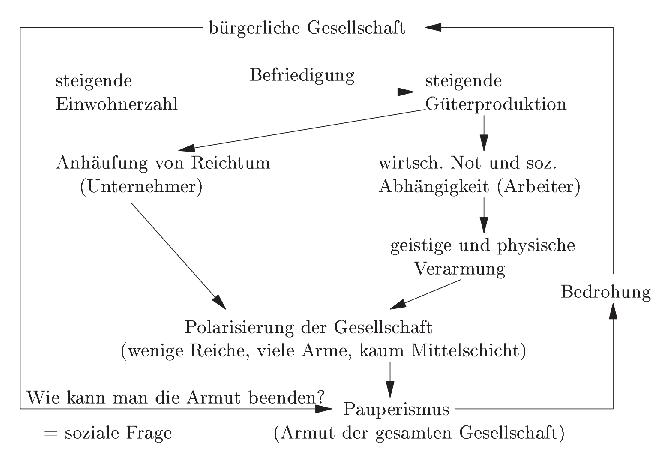
\includegraphics[width=\textwidth]{soz-frag-sch.eps}
\caption{Entstehung der sozialen Frage nach \Nam{}{Hegel}}
\label{pic:soz-frag-sch}
\end{figure}

\begin{figure}
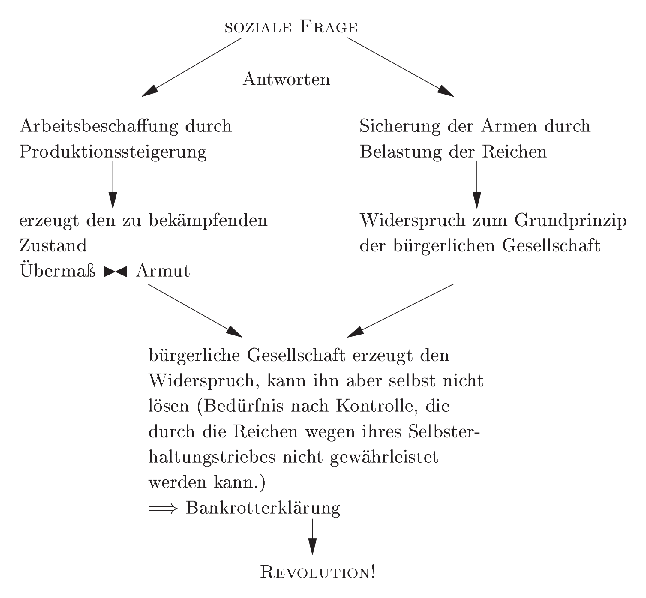
\includegraphics[width=\textwidth]{soz-frag-sch-rev.eps}
\caption{Folgen der sozialen Frage nach \Nam{}{Hegel}}
\label{pic:soz-frag-sch-rev}
\end{figure}

\endinput

\section{Lösungsansätze für die soziale Frage}
\label{sec:soz-frag-loes}
\index{soziale Frage!Lösungsansätze}

\begin{aufgabe}
Stellen Sie einen Maßnahmenkomplex zur Abmilderung/Lösung der Sozialen
Frage vor und prüfen Sie seine Wirksamkeit anhand Hegels Auffassungen! 
\end{aufgabe}

\subsection{Der Marxismus -- Veränderung durch Umbruch}
\label{ssc:marxismus}
\index{Marxismus}
\index{Materialismus}
\mar{\cite{DudPolGes} bietet hier eine gute Darstellung.}

\begin{aufgabe}
Erarbeiten Sie aus der Quelle Marx' Sicht auf die Rolle der
Bourgeoisie in der Geschichte!

Untersuchen Sie die Richtigkeit der fettgedruckten Position anhand des
kapitalistischen Produktionsprozesses in Marx' sogenannter \jar{Basis}! 

Überprüfen sie anhand des Hegelschen Systems der Sozialen Frage,
inwiefern die Ideen Marx' eine Lösung dieser darstellen!
\end{aufgabe}

Im Hefter ist dies in vorerst ausreichender Form dargestellt.

%%%%%%%%%%%%%%%%%%%%%%%%%%%%%%%%%%%%%%%%%%%%%%%%%%%%%%%%%%%%%%%%%%%%%%

\subsection{Die Arbeiterschaft -- Hilfe zur Selbsthilfe}
\label{ssc:arb-bew}
\label{ssc:soz-frag-loes-arb}
\index{Arbeiterbewegung}

\begin{aufgabe}
Untersuchen Sie, inwiefern die Gewerkschaften zur Lösung der sozialen
Frage beitrugen!
\end{aufgabe}

\subsubsection{Ausgangspunkt}

Der Vorteil der Arbeiter war, daß sie eine äußerst breite Schicht der
Bevölkerung bildeten. Unter der Voraussetzung, daß sie sich
zusammenschließen und als die Masse handeln, die sie waren, kann man
ihnen große Chancen, ihre Ziele und Interessen durchzusetzen,
einräumen.

Genau diese Voraussetzung ist aber das Problem, denn die Arbeiter
waren keine homogene Masse. Vielmehr gab es auch hier eine soziale
Schichtung, die sich in der Gehaltsstruktur ausdrückte und zum
ständigen Konflikt beispielsweise zwischen Meistern und
\glq{}Angelernten\grq{} führte. Das ständig bereitstehende
\emph{Ersatzheer} führte zu großer Konkurrenz untereinander. Dieses
Konfliktpotential wurde noch durch die Fabrikordnungen vergrößert,
denn diese sahen Kollektivstrafen vor.

Zur unterschiedlichen sozialen kam noch die unterschiedliche regionale
Herkunft. Da es der Arbeiterschaft an organisatorischem Wissen fehlte,
war es auch hier schwer, eine breite Basis für die Durchsetzung der
Ziele zu finden.

Die Lebensumstände der Arbeiter waren weiterhin schon so miserabel,
dass diese entweder gar keine Zeit fanden, sich um andere Probleme als
ihre eigenen, zu kümmern oder die ständigen Sorgen von vornherein in den
Alkohol oder den Sport flohen.\\


\subsubsection{Entwicklung der Arbeiterbewegung in Großbritannien}
\index{Arbeiterbewegung!Großbritannien}

\begin{chronik}
\item[nach 1814/15] zunehmende Politisierung des Aufbegehrens der
Arbeiter, Streiks

\item[1824] Aufhebung des Koalitionsverbots, Bildung von
Gewerkschaften und Gewerkschaftsverbänden in der Folge

\item[1840] Aus der chartistischen\footnote{Der Name \emph{Chartismus}
leitet sich aus dem Gesetzentwurf ab, der dieser Strömung entstammte
und Forderungen nach beschränkungslosen (Zensus etc.) jährlichen
geheimen allgemeinen Wahlen, Diäten für Abgeordnete und anderem
umsetzen sollte.} Strömung entstand die \ins{National
Chartist} als erste allerdings illegale Arbeiterpartei unserer Zeit.

\item[1860] Nachdem die politische Richtung der Arbeiterbewegung ins
Stocken gekommen war, bildet sich aus den entstehenden \emph{Trade
Unions} (Gewerkschaften) der \ins{Trade Union Council}.

\item[1864] Gründung der \ins{Internationalen
Arbeiterassoziation}\footnote{\Nam{Marx, Karl}{Karl Marx} war
eines der führenden Mitglieder.} (IAA) als Zusammenschluss aller
Arbeiterorganisationen

\item[1876] Auflösung der IAA nach Erfüllung ihrer Aufgabe,
Fortsetzung der Arbeit in Parteien
\end{chronik}


\subsubsection{Arbeiterparteien in Deutschland}
\index{Arbeiterparteien!Deutschland}
\mar{Zur Entwicklung siehe vorerst das Organigramm im Hefter.}

Ziele/Forderungen:

\begin{itemize}
\item Brechung des \Beg{Ehernes Lohngesetz}{Ehernen
Lohngesetzes}\footnote{Da \cite{WiLexEhLohnGes} eine andere Definition
bringt, als ich im Glossar niedergeschriebenen habe, ist fraglich, ob
der hier abgedruckte Sachverhalt stimmt.}
\item allgemeine, gleiche, direkte Wahl (Druckmittel gegen
Unternehmer)
\item Befreiung der Arbeiterklasse durch die Arbeiterklasse
\item Besetitigung der Abhängigkeit des Lohnarbeiters
\item politische Freiheiten (Voraussetzung für ökonomische
Freiheiten)
\item marxistische Strömungen: Revolution \index{Marxismus}
\item politisch-praktische Strömungen: Reformen
\end{itemize}

Mittel:

\begin{itemize}
\item Parteibildung und -arbeit
\item Wahlrechtskämpfe
\item Zusammenschluss von Arbeiterorganisationen
\item Gründung von Arbeiterproduktivgenossenschaften (Vorschlag
\Nam{Lassalle, Ferdinand}{Lassalle}s) -- Arbeiter selbst als
Unternehmer
\item Programme, Zeitschriften
\end{itemize}


\subsubsection{Gewerkschaften in Deutschland\mycite{MustaGeGe}}
\index{Gewerkschaften!Deutschland}

Die deutsche Gewerkschaftsbewegung wies einige Unterschiede zu der in
Großbritannien auf. So wurde in Deutschland durch späte Einführung des
Koalitionsrechts und Sozialistengesetz ein erheblicher Druck ausgeübt.
Dies führte dazu, dass die Vereinigungen im Untergrund
weiterexistieren mussten. Dadurch zu kluger Planung und Organisation
gezwungen, erfuhren die Gewerkschaften eine Stärkung.

Weiterhin waren die deutschen Gewerkschaften ideologisch breiter
aufgestellt. Das bedeutete natürlich, dass alle ihre
Interessenvertretung fanden, hatte aber auch den Nachteil, dass die
Möglichkeiten, als Masse zu handeln, eingeschränkt waren.

Letztendlich legte man in Deutschland sehr großen Wert auf die
organisatorische Trennung zwischen Gewerkschafts- und Parteiarbeit.
-- Die Gewerkschaften übernahmen die überparteiliche soziale
Unterstützung und Basisarbeit während politische und parlamentarische
Arbeit den Parteien zufiel. Man suchte so, die Sorge für die Lage der
Arbeiter unabhängig von politischen Meinungsverschiedenheiten zu
machen, rief die Arbeiter aber gleichzeitig auf, durch Parteieintritt
den Einfluss des Proletariats auf das Staatsgeschehen zu
vergrößern.\mycite{ResErfGeKo} \mycite{ResKonfGeVoGo}\\

\noindent Entwicklung:

\begin{chronik}
\item[nach 1848/49] lokale Arbeiterkomitees und -zusammenschlüsse

\item[1868] Gründung des \Ins{Allgemeiner Deutscher
Arbeiterschaftsverband}{Allgemeinen Deutschen
Arbeiterschaftsverbandes}

\item[1868] Gründung der \Ins{}{\Nam{Hirsch, Max}{Hirsch}-\Nam{Duncker,
Franz}{Duncker}schen-Gewerksverbände}\footnote{\cite{LEMOHiDu} datiert
hier auf 1869.}

\item[1869] Gründung der \Ins{Internationale
Gewerksgenossenschaften}{Internationalen Gewerksgenossenschaften}
durch \Nam{Bebel, August}{August Bebel} und \Nam{Liebknecht,
Wilhelm}{Wilhelm Liebknecht}

\item[1869] Koalitionsfreiheit für Preußen

\item[1878] \ges{Gesetz gegen die gemeingefährlichen Bestrebungen der
Sozialdemokratie} -- Weiterexistenz im Untergrund

\item[1886] Streikerlass in Preußen -- Verfolgung illegaler
Gewerkschaften

\item[1890] Aufhebung des Sozialistengesetzes

\item[1890] Gründung der \ins{Generalkommission der Freien
Gewerkschaften Deutschlands} als erster Dachorganisation für
sozialistische Gewerkschaften auf Initiative von \Nam{Legien,
Carl}{Carl Legien}

\item[1891] Gründung des \Ins{Deutscher
Metallarbeiterverband}{Deutschen Metallarbeiterverbandes} -- erste
Industriegewerkschaft

\item[1890er] Gründung christlicher Gewerkschaften, Formierung zum
Verband \mar{Irgendwie stimmen hier einige Zahlen nicht.}
\end{chronik}

Ziele:

\begin{itemize}
\item soziale Ziele --Loslösung von politischen Fragestellungen
\item kürzere Arbeitszeit
\item höhere Löhne
\item Abbau der Frontstellung des Proletariats gegen das Bürgertum
(Hirsch-Duncker)
\item Förderung und Wahrung der Würde und des materiellen Interesses
der Arbeiter
\end{itemize}

Mittel:

\begin{itemize}
\item Streik
\item lokale Komitees und Arbeiterzusammenschlüsse $\longrightarrow$
Gewerkschaften $\longrightarrow$ Gewerkschaftsverbände
\item Presseorgane
\item Kassen zur Unterstützung von Arbeitslosen, Not leidenden,
Kranken, Invaliden, Alten, Wandernden
\end{itemize}

\newpage
%%%%%%%%%%%%%%%%%%%%%%%%%%%%%%%%%%%%%%%%%%%%%%%%%%%%%%%%%%%%%%%%%%%%%%

\subsection{Die Rolle der Unternehmer}
\label{ssc:soz-frag-loes-unt}

\subsubsection{Maßnahmen}

% Breite der ersten Spalte der Tabelle
\newlength{\frstcol}
\settowidth{\frstcol}{\textsc{Harkort}}
\addtolength{\frstcol}{1ex}

% Breite der zweiten und dritten Spalte der Tabelle
\newlength{\sndthrdcol}
\newlength{\wholecols} % Breite von zweiter und dritter Spalte zusammen
\setlength{\wholecols}{\textwidth}
\addtolength{\wholecols}{-\frstcol}
\addtolength{\wholecols}{-5\tabcolsep}
\setlength{\sndthrdcol}{0.5\wholecols}



\tablefirsthead{
\toprule
Untern. & fürsorglicher Charakter & unterdrückender Charakter \\
\midrule}
\tablelasttail{\bottomrule}

\begin{supertabular*}{\textwidth}%
{p{\frstcol}p{\sndthrdcol}p{\sndthrdcol}}
\vspace{0.01pt}
\Nam{Stumm-Halberg, Carl Ferdinand Freiherr von}{Stumm}
& \begin{tablist}
\item Schulen
\item Verantwortlichkeit für außerfabrikale Arbeiterhandlungen
\item Ausschluss von Kinderarbeit
\item niedrigvermietete Werkswohnungen
\item Bibliotheken, Park für die Arbeiter, Militärkapellen
\item Kantinen, Teuerungszulagen
\item Bestrafungs- und Entlassungserlaubnis
\item Sprechstunden für die Belegschaft
\item überdurchschnittliche Löhne
\item protektorale Betriebsverfassungen
\end{tablist}
\noindent $\Longrightarrow$ Schutz der Arbeiter
& \begin{tablist}
\item Heiratserlaubnis nach Eigenschaften und Gesundheit der Partner,
Vorbeugung von Arbeitsausfall während Schwangerschaften
\item Erziehungsüberwachung
\item Zwang zum Kirchenbesuch
\item Arbeiter als geborene Untertanen (\emph{König Stumm})
\index{König Stumm}
\end{tablist}
\noindent $\Longrightarrow$ Eindringen in das Privatleben
\\

\vspace{0.01pt}
\Nam{Krupp, Alfred}{Krupp}
& \begin{tablist}
\item überdurchschnittliche Löhne
\item Betriebskrankenkasse
\item Sterbegelder an Hinterbliebene
\item Werkswohnungen
\item Arbeiterpensionskasse -- Altersabsicherung
\item \ins{Gemeinschaft der Kruppianer} -- Stammbelegschaft
\end{tablist}
& \begin{tablist}
\item Nutzung des \beg{Ersatzheeres}
\item Entlassung als Druckmittel
\item Entlassung bei Parteihörigkeit
\item Betäubung von sozialdemokratischen und gewerkschaftlichen
Bestrebungen
\item leistungsabhängige Entlohnung
\item Strafgelder
\item Beitrittspflicht zur Betriebskrankenkasse
\end{tablist}
\\

\vspace{0.01pt}
\Nam{Harkort, Friedrich}{Harkort}
& \begin{tablist}
\item betriebsinterne Sparkassen -- Sicherung von Grunderwerb
\item Bildungssystem für Kinder und Erwachsene -- geistliche,
sittliche und staatsbürgerliche Bildung seiner Angestellten
\item Ablehnung von Kinderarbeit
\end{tablist}
&\vspace{0.01pt} keine klassische Unterdrückung
\\
\end{supertabular*}

\ \\

Ein weiteres bedeutendes Unternehmen, in dem man die Lage der Arbeiter
zu bessern versuchte, war \ins{Carl Zeiss Jena}. Dabei waren die
dortigen Maßnahmen einmal und auch völlig andere als bei den oben
Aufgeführten.

\endinput



\chapter[Fortentwicklung der Industrialisierung in der ersten Hälfte
des 20. Jh.] {Fortentwicklung der Industrialisierung in der ersten
Hälfte des 20. Jahrhunderts}
\label{chp:fortentw-indust}

\section{Neue gesellschaftliche Schichtung}
\label{neue-ges-schicht}
\index{Gesellschaft}
\index{Agrargesellschaft}
\index{Industriegesellschaft}
\index{Dienstleistungsgesellschaft}

Die Gesellschaft in Deutschland entwickelte sich seit dem \dat{Ende der
Agrargesellschaft 1850} über die Industriegesellschaft zur
\dat{Dienstleistungsgesellschaft ab 1990}.

Dabei kann man drei große Linien erkennen: \emph{Urbanisierung}
\index{Urbanisierung}, \emph{Trennung von Arbeit und Leben}
beziehungsweise Hausgemeinschaft und Arbeitsstätte und eine zunehmende
\emph{Differenzierung der Arbeitnehmergesellschaft} in \beg{Arbeiter}
und \beg{Angestellte}. Außerdem setzte um 1900 die Bürokratisierung
ein. \index{Bürokratisierung} 

\endinput

\section{Neue Leitsektoren}
\label{sec:neue-leits}
\index{Leitsektor}

\subsection[Chemische Industrie]{Chemische Industrie\footnote{Die
Grundlage dieses Abschnitts ist ein schnell im Rahmen des Unterrichts
im Internet recherchierter Kurzvortrag. Da dieses Thema weniger
relevant ist, beschränke ich mich bei der Literatur auf die
Wikipedia-Artikel \cite{WikChemInd}, \cite{WikFarbst}, \cite{WikHaBoVerf}, \cite{WikStaudi} und \cite{WikSteikohteer}.}}
\label{ssc:chem-ind}
\index{Chemische Industrie}

\mar{Warum galt die chemische Industrie in jener Zeit als Friedens-
und damit Staatserhaltend?}
In der ersten Hälfte des 19. Jahrhunderts wurden Verfahren erfunden,
den bei der Gasherstellung anfallenden \emph{Steinkohlenteer}
\index{Steinkohlenteer} nutzbringend zu verwenden. Die neuen Produkte
-- allen voran \emph{Anilin} und \emph{Phenol}
\index{Anilin}\index{Phenol} -- waren Grundstoff für zahlreiche
Synthesen. -- Damit war der Aufstieg der Farbenindustrie eingeleitet.

Es wurden Möglichkeiten gefunden, Medikamente, Düngemittel und
Sprengstoffe künstlich herzustellen. Dadurch konnten bisher unheilbare
Krankheiten geheilt und die landwirtschaftliche Produktion erheblich
gesteigert werden. -- Gesundheits- und Versorgungszustand der
Bevölkerung verbesserten sich erheblich, sodass auch die Nachfrage
nach den immer vielseitigeren Produkten der chemischen Industrie
stieg.

Die enge Kooperation dieses Industriezweigs mit technischen
Hochschulen verbesserte das Bildungssystem und trieb die Forschung
voran. So kam es zu weiteren bedeutenden Erfindungen:

\dat{1910} wurde das \dat{\emph{\Nam{Haber, Fritz}{Haber}-\Nam{Bosch,
Carl}{Bosch}-Verfahren}} \index{Haber-Bosch-Verfahren} erfunden,
welches die Synthese von Ammoniak ermöglichte. Dieser dient als
Grundlage für Sprengstoffe und Kunstdünger. Die Verfügbarkeit neuer
Düngemittel bewirkte neue Forschungen in der Landwirtschaft.

\dat{1922} stellte \Nam{Staudinger, Hermann}{Hermann Staudinger} die
These auf, dass Polymere aus Makromoleküle bestehen und begründete
damit die Polymerchemie. Dies führte zur \dat{großtechnischen
Produktion zahlreicher Kunststoffe ab 1930} (beispielsweise
Polystyren, Polyvinylchlorid, Nylon, Buna). Die \dat{1925 gegründete}
\beg{IG Farben} war hier marktführend.

%%%%%%%%%%%%%%%%%%%%%%%%%%%%%%%%%%%%%%%%%%%%%%%%%%%%%%%%%%%%%%%%%%%%%%

\subsection[Elektroindustrie]{Elektroindustrie\footnote{Dieser und die
folgenden vier Abschnitte entstammend Kurzvorträgen, die ich nicht
selbst gehalten habe und deswegen auch keine Quellen angeben kann.}}
\label{ssc:el-ind}
\index{Elektroindustrie}

\begin{chronik}
\item[ab 1900]
erste kommerzielle Sende- und Empfangsanlagen

\item[1904]
erste Röhrendiode -- Gleichrichtung\index{Röhrendiode}

\item[1906]
erste Triode -- Grundlage für Radio und andere Unterhaltungselektronik 
\index{Triode}

\item[1926\,--\,1931] Entwicklung des Fernsehens\index{Fernsehen}

\item[1900\,--\,1950] auch international marktbeherrschende Stellung
von \beg{AEG} und \beg{Siemens}

\item[1931]
Erfindung des Elektronenmikroskops\index{Elektronenmikroskop}

\item[1941]
Erfindung des Computers (Z\,3)\index{Computer}\index{Z\,3}
\end{chronik}

Diese Entwicklungen läuteten des Computer- und Informationszeitalter
ein: Die neuen Möglichkeiten erweckten sofort großes in der
Bevölkerung, in der Politik und beim Militär, sodass sich die Anzahl
der Arbeitsplätze von \dat{80\,000 Beschäftigten 1900} bis \dat{1950
auf 650\,000} steigerte.

%%%%%%%%%%%%%%%%%%%%%%%%%%%%%%%%%%%%%%%%%%%%%%%%%%%%%%%%%%%%%%%%%%%%%%

\subsection{Fahrzeugbau}
\label{ssc:fahrzbau}
\index{Fahrzeugbau}

Sich aus dem Waggonbau entwickelnd erfuhr dieser Industriezweig in
Folge der \dat{Forderung \Nam{Hitler, Adolf}{Hitler}s} nach einem
Wagen für breite Schichten \dat{1934} großen Aufschwung. So wurde
\dat{1937} die \dat{\ins{Gesellschaft zur Vorbereitung der Deutschen
Volkswagen mbH} gegründet}, \dat{1938 in \ins{Volkswagen GmbH}}
umbenannt.

Das Werk wurde im gleichen Jahr in \ort{Wolfsburg}
errichtet.\index{VW} Es war äußerst günstig gelegen: In der Mitte
Deutschlands mit Anbindung an Autobahn, Eisenbahn und durch den
Mittellandkanal ebenfalls an Wasserstraßen. Außerdem waren Stahlwerke,
beispielsweise in \ort{Salzgitter} nicht fern. Im Krieg leisteten hier
20\,000 Kriegsgefangene und KZ-Insassen Zwangsarbeit.
\index{Zwangsarbeit}

Bei der Produktion des neu entwickelten
\emph{KdF-Wagens}\index{KdF-Wagen}, heute als \emph{VW Käfer}\index{VW
Käfer} bekannt, orientierte man sich am
\emph{Fließbandbetrieb}\index{Fließbandproduktion}, wie er bei
\ins{Ford} in \ort{Detroit} praktiziert wurde. Das neue Auto konnte
vier Personen transportieren, war zuverlässig, einfach reparierbar und
billig. So konnte man die Wirtschaft ankurbeln und die Verwendung beim
Militär war auch möglich.  Im Krieg stand dann auch die
Rüstungsproduktion im Vordergrund.  \index{Rüstung}

Nach dem Krieg war das VW-Werk der britischen Militärregierung
\index{Militärregierung} unterstellt, die die Umstellung auf
Zivilproduktion veranlasste.

\endinput

\section{Fließbandarbeit}
\label{ssc:fliessbarb}
\index{Fließbandarbeit}

Die Arbeitswelt in der ersten Hälfte des 20. Jahrhunderts war geprägt
vom \beg{Taylorismus}, der in Kombination mit dem Fließbandbetrieb die
Massenproduktion ermöglichte.

Dieses neue Prinzip der Trennung von geistiger und körperlicher Arbeit
half bei der Lösung sozialer Probleme und versprach \jar{Wohlstand für
alle}. Der anfängliche Enthusiasmus wich aber bald der
Unzufriedenheit: Durch die Monotonie der Arbeit stellten sich
gesundheitliche Probleme ein. Außerdem konnten sich die Arbeiter nun
kaum noch mit ihrem Betrieb und den Erzeugnissen identifizieren, weil
sie das Endprodukt kaum noch zu Gesicht bekamen.

Die Qualität litt und die Motivation fehlte. Es kam zu Konflikten mit
den Arbeitgebern; wo es möglich war wanderten die Arbeitnehmer in den
Dienstleistungssektor ab.

\endinput

\section{Arbeitsbedingungen in der ersten Hälfte des 20. Jahrhunderts}
\label{sec:arb-bed-20jh}

Die Arbeitswelt in der ersten Hälfte des 20. Jahrhunderts war auch
geprägt von miserablen Arbeitsbedingungen: \emph{Niedrige
Mindestanforderugen}, \emph{fehlende Aufstiegschancen}, 
\emph{hohe Fluktuation}, \emph{niedrige Löhne} und \emph{geringe
Arbeitsplatzsicherheit} machten den Arbeitern das Leben schwer.

Doch man tat auch einiges, um jene Bedingungen zu verbessern.  Gab es
um \dat{1900} wenigstens einige \dat{Herbergen für Wanderarbeiter},
brachte das \dat{\emph{\Nam{Stinnes, Hugo}{Stinnes}-\Nam{Legien,
Carl}{Legien}-Abkommen} vom 15.\,11.\,1918} große Fortschritte. Der
aus Furcht vor einer Vergesellschaftung der deutschen Industrie im Zuge
der Novemberrevolution zwischen Gewerkschafts- \Nam{}{Legien} und
Industrievertretern \Nam{}{Stinnes} geschlossene Vertrag legte die
Zusammenarbeit von Arbeitnehmern und -gebern fest. Die Arbeitgeber
verpflichteten sich so, die Rolle der Gewerkschaften als Vertreter der
Arbeiterinteressen anzuerkennen und sie als gleichberechtigte
Tarifpartner zu betrachten. Außerdem wurde der \emph{Achtstundentag}
bei vollem Lohnausgleich eingeführt.
\index{Arbeitnehmer}
\index{Arbeitgeber}
\index{Gewerkschaft}
\index{Tarifverhandlung}
\index{Achtstundentag}

Damit wurden ab 1918/1919 in allen Branchen \emph{Tarifverträge},
Regelung der Arbeitsbedingungen durch \emph{Kollektivvereinbarungen},
Anerkennung der \emph{Koalitionsfreiheit} durch die Arbeitgeber und
\emph{Arbeiterausschüsse} in Betrieben mit mindestens 50 Beschäftigten
möglich.
\index{Tarifvertrag}
\index{Kollektivvereinbarung}
\index{Koalitionsfreiheit}
\index{Arbeiterausschuss}

\endinput



\chapter[Ursprung und Umsetzung liberaler, nationaler und
kons. Ideen im 19. Jh.]{Ursprung und Umsetzung liberaler und
nationaler sowie konservativer Ideen im 19. Jahrhundert\footnote{Ich
stütze mich bei der Strukturierung dieses Kapitels ausnahmsweise kaum
auf den Hefter, da dort keine erkennbare Struktur existiert.}}
\label{chp:lib-nat-kons}

Dieses Kapitel soll folgende Fragen beantworten:

\textbf{Warum kommt es zur Revolution?}

\textbf{Welche Forderungen haben die Bürger?}

\textbf{Warum haben die Bürger gerade diese Forderungen?}

\section{Die Epoche der Aufklärung}
\label{sec:aufkl}
\index{Aufklärung}

Die Ideen der Aufklärung bildeten die Grundlage für die politischen,
ökonomischen und sozialen Entwicklung, die schließlich zur Revolution
von 1848 führten. Sie beeinflussten außerdem seit Mitte des 18.
Jahrhunderts das Denken aller Menschen in Europa und Nordamerika und
sind bis heute gültig und wirksam.

Dieser Abschnitt soll einen kurzen Überblick über die für das Weitere
relevanten Aspekte der Aufklärung geben.


\subsection{Konflikt mit der alten Ordnung}

% wieder mal Spaltenbreiten berechnen

\begin{tabularx}{\textwidth}{XcX}
\toprule
Situation in Deutschland vor 1815 &
&
Ziele der Aufklärung \\

\midrule
\vspace{-45mm}
\begin{tablist}
\item absolutistische Monarchie 
\item Ständegesellschaft
\item territorialstaatlicher Absolutismus -- Vielzahl von
Einzelstaaten
\item Leibeigenschaft (Bindung als Person)
\item Schollenbindung (Bindung als Pacht)
\item Zünfte/Gilden
\end{tablist}
&
\unitlength=2.5mm
\begin{picture}(3,19)
\thicklines
\put(2,18){\line(-2,-9){2}}
\put(0,9){\line(3,1){3}}
\put(3,10){\vector(-2,-9){2}}
\end{picture}
&

\vspace{-45mm}
\begin{tablist}
\item Vernunftorientierung 
\item gegen Dogmatik der Kirche
\item mündiger Bürger
\item geistige und persönliche Freiheit
\item Toleranz (Religionstoleranz)
\item politisches Mitspracherecht
\end{tablist}
\\

\bottomrule
\end{tabularx}

%%%%%%%%%%%%%%%%%%%%%%%%%%%%%%%%%%%%%%%%%%%%%%%%%%%%%%%%%%%%%%%%%%%%%%

\subsection{Leistungen}

Zu einer sehr komprimierten Übersicht über die Leistungen der
Aufklärung siehe Tabelle \ref{tab:leist-aufkl}.

% angenehme Breite der ersten Spalte
\settowidth{\tymin}{\textbf{Natur-}}

\begin{sidewaystable}
\label{tab:leist-aufkl}
\caption{Leistungen der Aufklärung}
\footnotesize
\renewcommand{\arraystretch}{1.5}

\begin{tabulary}{\textheight}{LLLL}
\toprule

&
\textbf{Die alte Ordnung} &
\textbf{Die Ideen der Aufklärung} &
\textbf{Anwendung der neuen Erkenntnisse} \\

\midrule

\textbf{Naturwissenschaft} &
Spekulation \newline
Überlieferung &
empirische Methode (\Nam{Newton, Sir Isaac}{Newton}): Beobachtung --
Verallgemeinerung bzw. Experiment -- Erkenntnis \newline
einzige Grundlage: \emph{Vernunft} &
\Nam{Newton, Sir Isaac}{Newton}: Gravitationsgesetz \newline
\Nam{Kepler, Johannes}{Kepler}: Gesetze der Planetenbewegung \newline
\Nam{Watt, James}{Watt}: Dampfmaschine \newline
Diese und zahlreiche weitere Erfindungen bringen großen technischen
Fortschritt. Wissenserweiterung und Bildung gewinnen an Bedeutung.
\\

\textbf{Gesellschaft} &
Ständegesellschaft &
natürliche Freiheit und Gleichheit der Menschen (\Nam{Locke,
John}{John Locke}) &
Formulierung der Menschenrecht \\

\textbf{Religion} &
Gott und die Bibel als alleinige Autorität &
von Gott nach vernünftigen Gesetzen geschaffene Welt \newline
Religionsfreiheit &
Toleranz zwischen den Religionen \\

\textbf{Politik} &
Gottesgnadentum -- Absolutheitsanspruch des Herrschers &
Kontrolle des Herrschers durch die Bürger (\Nam{Montesquieu, Baron
de}{Montesquieu}, \Nam{Rousseau, Jean-Jacques}{Rousseau}) &
Gewaltenteilung, demokratische Verfassung, Volkssouveränität \\

\textbf{Wirtschaft} &
staatlich gelenkte Wirtschaft &
Wohlstand aller Bürger des Staates durch wirtschaftliche Freiheit des
Einzelnen (\Nam{Smith, Adam}{Smith}) &
Wirtschaftsliberalismus \\

\bottomrule 
\end{tabulary}
\end{sidewaystable}

%%%%%%%%%%%%%%%%%%%%%%%%%%%%%%%%%%%%%%%%%%%%%%%%%%%%%%%%%%%%%%%%%%%%%%

\subsection{Philosophen der Aufklärung}

Es gab zahlreiche Philosophen, die die Ideen der Aufklärung
entwickelten und verfolgten, darunter zum Beispiel \Nam{Leibniz,
Gottfried Wilhelm}{Leibniz}, \Nam{Kant, Immanuel}{Kant}, \Nam{Herder,
Johann Gottfried}{Herder}, \Nam{Lessing, Gotthold Ephraim}{Lessing}.
Im Folgenden wird jedoch nur Einblick in die Philosophie zweier Männer
gegeben, die sich besonders mit Staatstheorien beschäftigt haben und
deshalb für dieses Kapitel relevant sind.


\subsubsection{\Nam{Montesquieu, Baron de}{Charles de Secondat, Baron
de Montesquieu}}
\index{Gewaltenteilung}
\index{Legislative}
\index{Exekutive}
\index{Judikative}
\index{politische Freiheit}

\Nam{}{Montesquieu} geht in seinem Werk \emph{Vom Geist der
Gesetze}\mycite{VomGeistderGes} unter anderem auf die Frage ein, wie
ein Staat gestaltet sein muss, damit die politische Freiheit der
Bürger gewährleistet ist. Dabei definiert er \jar{politische Freiheit}
als \textquote{jene geistige Beruhigung, die aus Überzeugung
hervorgeht, die jedermann von seiner Sicherheit hat}.

Er stellt dazu fest, dass es in jedem Staat drei Gewalten gibt, die
wir heute \emph{Legislative} (Erlassen von Gesetzen), \emph{Exekutive}
(Umsetzung öffentlicher Beschlüsse) und \emph{Judikative}
(Verhandlung von Streitfällen und Verbrechen). Um also die politische
Freiheit des Bürgers zu sichern, ist es essentiell, dass jene Gewalten
personell strikt voneinander getrennt werden:

\SetBlockThreshold{0}
\blockquote[{\mycite[216\,f.]{VomGeistderGes}\,\footnote{Der
Quellenverweis gilt auch für den obigen Abschnitt.} }]{Alles wäre
verloren, wenn ein und derselbe Mann beziehungsweise die gleiche
Körperschaft entweder der Mächtigsten oder der Adligen oder des Volkes
folgende drei Machtvollkommenheiten ausübte: Gesetze erlassen,
öffentliche Beschlüsse in die Tat umsetzen, Verbrechen und private
Streitfälle aburteilen.}


\subsubsection{\Nam{Rousseau, Jean-Jacques}{Jean-Jacques Rousseau}}
\index{Grundrechte}
\index{Menschenrechte}
\index{Französische Revolution}

\blockquote{Der Mensch wird frei geboren, und dennoch liegt er in
Ketten.}

\blockquote[{\mycite{DerGesVertr}\,\footnote{Ich beziehe mich in
diesen Zitaten und in den folgenden Ausführungen auf den mir
vorliegenden Text. Dieser ist allerdings aus verschiedenen Teilen des
Werkes zusammengestückelt und weder mit Auslassungsmarken, noch mit
einer Quellenangabe versehen. Mit \cite{DerGesVertr} ist damit ein
Hinweis auf eine Volltextfassung gegeben, die allerdings im Wortlaut
nicht exakt meinem Text entspricht.}}]{Auf seine Freiheit verzichten,
heißt auf seine Eigenschaft als Mensch, auf die Menschenrechte, sogar
auf seine Pflichten zu verzichten.}

Wie man an diesen Zitaten erkennen kann, legt \Nam{}{Rousseau}
besonders großen Wert auf Freiheit. Deshalb setzt er auf seiner Suche
nach einer Gesellschaftsform, die Person und Eigentum eines jeden
schützt, also Grund- und Menschenrechte garantiert, die Prämisse, dass
der Mensch in dieser Gesellschaft den gleichen Grad an Freiheit
genießt, wie außerhalb\footnote{Das ist im
\emph{Naturzustand}\index{Naturzustand}}.  Das Ergebnis von
\Nam{}{Rousseau}s Überlegungen ist der \ges{Gesellschaftsvertrag},
welcher die Voraussetzungen erfüllt und den Rahmen für die
Zusammensetzung der Gesellschaft festlegt: Jedes Mitglied der
Gemeinschaft gibt sich mit all seinen Rechten an die Gesellschaft hin.

Inwiefern diese Auffassung utopisch beziehungsweise realistisch ist,
ist eine andere Frage. Dennoch sind die Ideen, die \Nam{}{Rousseau}
hier formuliert, essentiell und waren eine äußerst wichtige geistige
Grundlage für die \emph{Französische Revolution}.


\subsubsection{Zusammenfassung: Wesentliche Ordnungsvorstellungen der
Aufklärer}
\index{Gewaltenteilung}
\index{Volkssouveränität}
\index{Grundrechte}
\index{Menschenrechte}

\begin{enumerate}
\item  das Prinzip der \emph{Gewaltenteilung}, das die Trennung von
ausführender und gesetzgebender Gewalt sowie die Sicherung einer
unabhängigen Rechtssprechung vorsieht
\item das Prinzip der \emph{Volkssouveränität}, das das Recht zur
Gesetzgebung den Vertretern des Volkes vorbehält
\item die Bindung des Gesetzgebers an allgemein gültige \emph{Grund-
und Menschenrechte}
\end{enumerate}

%%%%%%%%%%%%%%%%%%%%%%%%%%%%%%%%%%%%%%%%%%%%%%%%%%%%%%%%%%%%%%%%%%%%%%

\subsection{Umsetzung der Ideen der Aufklärung in der
\index{Französischen Revolution}}
\index{Bürgerrechte}
\index{Menschenrechte}
\index{Grundrechte}

\mar{Siehe Blatt mit schicken Unterstreichungen aus
dem Hefter.}
Während der die \dat{\ges{Erklärung der Bürger- und Menschenrechte}
von 1789} und in die \dat{französischen Verfassungen}, deren erste
\dat{1791} verabschiedet wurde, flossen zahlreiche Ideen der
Aufklärer, insbesondere \Nam{Montesquieu, Baron
de}{Montesquieu}s und \Nam{Rousseau, Jean-Jacques}{Rousseau}s ein. Die
Französische Revolution wiederum hatte großen Einfluss auf die
politischen Entwicklungen in Deutschland, die in diesem Kapitel
behandelt werden.

\endinput

\section[Nationale und liberale Bewegungen]{Nationale und liberale
Bewegungen\mycite{19Jh1}}
\label{sec:nat-lib-bew}
\index{nationale Bewegungen}
\index{liberale Bewegungen}

\mar{Belege aus IzpB?}
\subsection{Befreiungskriege gegen \Nam{Napol\'eon \Rm{1}}{Napol\'eon}}
\index{Befreiungskriege}
\index{Napol\'eonische Kriege}
\index{Nationalromantik}
\index{Nationalismus}
\index{Franzosenhass}

\mar{Muss das genauer gewusst werden?}
Der Begriff \emph{Befreiungskriege} steht hier für die Kriege
vornehmlich der von \Nam{}{Napol\'eon} besetzten Länder gegen die
französische Fremdherrschaft in der Zeit zwischen dem \dat{Rückzug der
\emph{Grande Arm\'ee} aus Russland 1812} und der \dat{Abdankung des
Kaisers 1814}. Jene Erfahrungen, die des gemeinsam geführte Krieges
und der Fremdherrschaft, waren eine wichtige Wurzel der
nationalen Bewegung, deren Formen von Nationalromantik bis zum
radikalen Nationalismus reichten. Ein verbreitetes Symptom war auch
der teils extreme Hass auf Franzosen.


\subsubsection{Ausgangslage}

Der \dat{Russlandfeldzug} und die
einhergehende Niederlage der Grande Arm\'ee hatten \dat{1812} Napol\'eon
gewaltige Verluste eingebracht.  Dadurch fasste Europa neuen Mut, eine
Befreiung von der französischen Herrschaft zu versuchen.


\subsubsection{Erhebung Preußens}

\begin{chronik}
\item[30.\,12.\,1812]
Unterzeichnung der \ges{Konvention von Tauroggen} als
preußisch-russisches Neutralitätsabkommen -- Anfang vom Ende der
erzwungenen militärischen Unterstützung Frankreichs durch Preußen

\item[28.\,2.\,1813]
Unterzeichnung des \Ges{Bündnis von Kalisch}{Bündnisses von Kalisch}
durch \nam{Wilhelm \Rm{3}} -- Zusammenarbeit Preußens und Russlands
für die Befreiung Europas

\item[10.\,3.\,1813]
erstmalige Verleihung des \emph{Eisernen Kreuzes} \index{Eisernes
Kreuz} durch Wilhelm \Rm{3}

\item[16.\,3.\,1813]
Kriegserklärung Preußens an Frankreich

\item[17.\,3.\,1813]
Aufruf \ges{An Mein Volk} von Wilhelm \Rm{3}\mycite{AnMeinVolk}
\end{chronik}


\subsubsection{Frühjahrsfeldzug 1813}
\index{Antinapoleonische Koalition}

\begin{chronik}
\item[2. und 20. Mai]
Schlachten bei \ort{Großgörschen} und \ort{Bautzen} -- Siege Napol\'eons

\item[12. Juli]
\emph{Trachenbergplan} \index{Trachenbergplan} -- gemeinsame Strategie
Preußens, Russlands und Schwedens gegen Napol\'eon

\item[11. August]
Kriegserklärung Österreichs an Frankreich. Zuvor waren Österreich,
Schweden und Großbritannien der Koalition gegen Napol\'eon beigetreten.
Deren Ziele waren die vollständige \emph{Wiederherstellung}
Österreichs und Preußens, die \emph{Unabhängigkeit} aller deutschen
Staaten sowie die Auflösung des \ins{Rheinbund}es.\footnote{Ich
vermute, dass das in dem Handout des Vortrags, der dieses Thema
behandelte, so gemeint war.}
\end{chronik}


\subsubsection{Herbstfeldzug 1813}

\dat{Ende August 1813} stießen drei russisch-schwedisch-preußische
Armeen unter österreichischem Oberbefehl gegen Napol\'eon vor:
\ins{Nordarmee} und \ins{Schlesische Armee} bei \ort{Dresden} und die
\ins{Hauptarmee} in \ort{Böhmen}.\footnote{Zumindest soweit ich das
Handout verstehe.}


\subsubsection{Weitere Schlachten 1813}
\index{Alliierte!Napol\'eonische Kriege}

\begin{chronik}
\item[23. Aug.] \ort{Großbeeren} -- Sieg der Alliierten
\item[26. Aug.] \ort{Katzbach} -- Sieg der Alliierten
\item[26./27. Aug.] \ort{Dresden} -- Sieg Napol\'eons
\item[20. Aug.] \ort{Kullm} und \ort{Nollendorf} -- Sieg der
Alliierten
\item[6. Sept.] \ort{Dennewitz} -- Sieg der Alliierten
\end{chronik}

In der Folge kündigte auch Bayern das Bündnis mit Napol\'eon und trat
der Koalition bei, was die Auflösung des Rheinbundes einleitete.

Mit der Umzingelung Napol\'eons bei \ort{Leipzig} kam es schließlich zur
\emph{Völkerschlacht}.


\subsubsection{Völkerschlacht bei Leipzig}
\index{Völkerschlacht}

Napol\'eon hatte sich mit stark geschwächtem Heer und knapper Munition
bei Leipzig aufgestellt. Die am \dat{16. Oktober 1813} beginnende
Schlacht verlief für die Alliierten erfolgreich. Der Sieg brachte den
Verlust des Rheinbundes und den Zusammenbruch der französischen
Herrschaft über Deutschland.

Da Napol\'eon jedoch am \dat{19. Oktober} rechtzeitig den
\dat{Rückzug} einleitete, konnte ein großer Teil seiner Armee
entkommen.


\subsubsection{Untergang Napol\'eons}

Die Alliierten marschierten nun in Frankreich ein und nahmen
\dat{\ort{Paris} am 31. März 1814}. Napol\'eon dankte ab und ging ins
Exil. Der \dat{\ges{Frieden von Paris} vom 30. Mai 1814} brachte das
vorläufige Ende der Napol\'eonischen Kriege.

%%%%%%%%%%%%%%%%%%%%%%%%%%%%%%%%%%%%%%%%%%%%%%%%%%%%%%%%%%%%%%%%%%%%%%

\subsection{Ausgangslage am Anfang des 19. Jahrhunderts}

War Deutschland bis 1871 keine Nation, existierte vor der
napol\'eonischen Besatzungszeit lediglich eine Vielzahl (über 100)
kleiner bis winziger Territorialstaaten. Zu einer Milderung dieses
Zustandes kam es durch Erscheinungen der \emph{Industrielle
Revolution}, durch \Nam{Napol\'eon \Rm{1.}}{Napol\'eon} selbst und im
Zuge der Befreiung von der französischen Fremdherrschaft:


\subsubsection[Veränderungen durch die Industrielle
Revolution]{Veränderungen durch die Industrielle Revolution (siehe
auch \ref{sec:aufh-rueckst-d})}

\begin{itemize}
\item Zollvereine: \ins{Allgemeiner deutscher Zollverein},
\ins{Zollvereinstaler}
\item Verbesserung der Infrastruktur (bspw. Eisenbahn) 
\item einheitlicher Markt
\end{itemize}


\subsubsection{Veränderungen durch
Napol\'eon\mycite[244-246]{gelbesGeschichts}}
\label{sss:veraend-nap}
\index{Flurbereinigung}
\index{Kleinstaaterei!Ende}

\begin{enumerate}
\item \emph{Flurbereinigung}:
Nachdem die linksrheinischen Fürsten ihre \dat{1801 Gebiete an
Frankreich abtreten} mussten, wurden sie durch den
\dat{\ges{Reichsdeputationshauptschluss} 1803} mit Land aus der von
Napol\'eon betriebenen \beg{Säkularisation} und \beg{Mediatisierung}
entschädigt.

\item \dat{Mediatisierung zahlreicher Reichsritterschaften 1805}

\item \dat{Gründung des \Ins{}{\beg{Rheinbundes}} 1806}:
In dieser Verwaltungseinheit von 16 deutschen Staaten führte Napol\'eon 
den \ges{Code civil} ein. Diese Gesetzessammlung galt bereits in
Frankreich, brachte liberale Reformen mit sich und bildete eine sich
über die Rheinbundstaaten erstreckende einheitliche Gesetzesgrundlage.
\end{enumerate}


\subsubsection{Veränderungen im Zuge der Befreiung von Napol\'eon}
\mar{Wo sind sie denn?}

%%%%%%%%%%%%%%%%%%%%%%%%%%%%%%%%%%%%%%%%%%%%%%%%%%%%%%%%%%%%%%%%%%%%%%

\subsection[Der Wiener Kongress 18. September 1814\,--\,9. Juni
1815]{Der Wiener Kongress 18. September 1814\,--\,9. Juni
1815\mycite[80\,--\,84, 88/89]{braunesGeschichts}\,\mycite[252\,--\,254]{gelbesGeschichts}}
\index{Wiener Kongress}
\index{Aufklärung}
\index{Nationalbewusstsein}

\begin{aufgabe}
Bewerten Sie anhand der Prinzipien den Charakter des Wiener
Kongresses! 
\end{aufgabe}

In deutschen Landen hatte sich während der Zeit der naol\'eonischen
Herrschaft einiges getan: Im \emph{territorialen Bereich} gab es
Veränderungen der Länder, der Grenzen und der Fürstentitel, in der
\emph{Wirtschaft} hatte sich der Markt vereinheitlicht und
\emph{politisch} gab es noch mehr Zündstoff: Die \emph{Aufklärung}
(siehe auch \ref{sec:aufkl} Griff um sich, die Befreiungskriege hatten
Anfänge eines \emph{Nationalbewusstseins} geschaffen und einige
Staatsleute begannen, der Entwicklung mit \emph{Reformen} beizukommen.

Um mit den Ereignissen Schritt zu halten, trafen sich 200 Vertreter
vieler europäischer Länder nach dem vorläufigen Sieg über Napol\'eon
in \ort{Wien} zu einem Kongress unter dem Vorsitz des \Nam{Metternich,
Klemens Wenzel Lothar von}{Fürsten von Metternich}.

Unter den zentralen Prinzipien

\begin{center}
\Large
%\begin{tabularx}{0.75\textwidth}{ccc}
%\textbf{\beg{Legitimität}} & \textbf{\beg{Solidarität}}
% & \textbf{\beg{Restauration}} 
%\end{tabularx}
\end{center}

\noindent berieten sie über die \emph{Neuregelung} europäischer
Grenzen und damit verbundenen territorialen \emph{Ausgleich}, über die
\emph{Fixierung} der Niederlage Frankreichs, politische
\emph{Regulierung} und ein europäisches
\emph{Sicherheitssystem}.\index{Sicherheitssystem} Damit einher ging
die Festsetzung der \emph{Pentarchie}, also die Voherrschaft der fünf
europäischen Großmächte Frankreich, Großbritannien, Österreich, Preußen 
und Russland in Europa.\index{Pentarchie}

An seinen Prinzipien eindeutig erkennbar, war der Wiener Kongress ein
Rückschritt in Bezug auf die nationale und liberalen Bemühungen in
deutschen Landen, wobei diese noch kaum begonnen hatten.

%%%%%%%%%%%%%%%%%%%%%%%%%%%%%%%%%%%%%%%%%%%%%%%%%%%%%%%%%%%%%%%%%%%%%%

\subsection{Nationale Bewegung}
\index{nationale Bewegungen}
\index{Einheit!19. Jahrhundert}
\index{Nationalstaat}

\noindent Wurzeln:

\begin{itemize}
\item die \emph{Französische Revolution}\index{Französische
Revolution} -- Die Leistungen, die die Menschen hier durch ihren
Patriotismus gebracht hatten, besonders natürlich die großen Erfolge
des materiell und personell Unterlegenen französischen Heeres, hatte
große Vorbildwirkung auf Deutschland.

\item die \emph{Preußischen Reformen} (siehe auch
\ref{sec:aufh-rueckst-d}) -- Sie erhöhten in den Befreiungskriegen
Kampfmoral und Bereitschaft zum Kampf und nährten die Hoffnung auf
einen Nationalstaat.

\item \Nam{Napol\'eon \Rm{1}}{Napol\'eon} als \emph{der} Übermittler
des Nationalbewusstseins -- das sich letztlich gegen ihn richtete.

\item Französische Fremdherrschaft und Ablehnung des
\jar{Franzosentums} betreiben die Bildung einer deutschen Identität.

\item der Aufruf \Nam{Wilhelm \Rm{3}}{Wilhelms \Rm{3}} \ges{An Mein
Volk}\mycite{AnMeinVolk}
\end{itemize}


\noindent Ziel:
\index{Kleinstaaterei!Ende}

Das zentrale Ziel der nationalen Bewegung war natürlich die Einheit
Deutschlands. Diese war zwar durch den \ins{Zollverein} (siehe
\ref{ssc:zollv} im wirtschaftlichen Bereich gegeben und Napol\'eon
hatte durch seine Flurbereinigung (siehe \ref{sss:veraend-nap})
der Kleinstaaterei ein Ende gesetzt. Dennoch konnte man nicht von
Deutschland als einem \emph{Nationalstaat} sprechen.


%%%%%%%%%%%%%%%%%%%%%%%%%%%%%%%%%%%%%%%%%%%%%%%%%%%%%%%%%%%%%%%%%%%%%%

\subsection{Liberale Bewegung}
\index{liberale Bewegungen}
\index{Gewaltenteilung}
\index{Volkssouveränität}
\index{Grundrechte}
\index{Menschenrechte}
\index{Gottesgnadentum!Abschaffung}

\noindent Ursprung:
\index{Gleichheit}
\index{Freiheit}
\index{Staatstheorie}
\index{Vertragstheorie}
\index{Gesellschaftsvertrag}
\index{Privateigentum}

Die Grundlage der liberalen Bewegungen war die bereits in Abschnitt
\ref{sec:aufkl} besprochene Aufklärung, die bekanntlich die Vernunft
ganz vornanstellt und an ihr Erkenntnis und Handeln bemisst. Über
diese gelangten dann auch die großen Vertrags- beziehungsweise
Staatstheoretiker \Nam{Locke, John}{John Locke}, \Nam{Montesquieu,
Baron de}{Baron de Montesquieu} und \Nam{Rousseau,
Jean-Jacques}{Jean-Jacques Rousseau}  mit ihren Ansätzen
genannt:\footnote{Natürlich gehört zu diesen auch \Nam{Hobbes,
Thomas}{Thomas Hobbes}. Doch dieser hat mit zur liberalen einer eher
unbedeutende Beziehung.} zu den Prinzipien, die auch zu den Prinzipien
der liberalen Bewegung wurden:

\begin{itemize}
\item Einführung eines Gesellschaftsvertrages zur eindeutigen
Festlegung der Rechte und Pflichten der Bürger und der Regierung eines
Landes und als Begründung beziehungsweise Legitimierung der Herrschaft
des regierenden Personenkreises -- kein \emph{Gottesgnadentum}
\item Volkssouveränität
\item Gewaltenteilung
\item Sicherung des Privateigentums
\item natürliche Gleichheit und Freiheit des Individuums
\item angeborene, unantastbare und unveräußerliche Grund- und
Menschenrechte
\end{itemize}


\noindent Zentrale Ziele:
\index{Feudalismus!Abschaffung}
\index{Wirtschaft!freie}
\index{Merkantilismus!Abschaffung}
\index{Wahl}

\begin{itemize}
\item Abschaffung der feudalen Gesellschaftsordnung 
\item Begrenzung der Fürstenmacht durch Verfassungen -- Anerkennung
von Grund- und Menschenrechten, Gewaltenteilung
\item Mitwirkung der Bürger durch gewählte Vertreter an der
Staatslenkung
\item freie Wirtschaft
\end{itemize}

Für die Erreichung dieser Ziele waren durch den \ges{Code civil} im
Rheinbund und die Reformen in Preußen zumindest Ansätze vorhanden.

%%%%%%%%%%%%%%%%%%%%%%%%%%%%%%%%%%%%%%%%%%%%%%%%%%%%%%%%%%%%%%%%%%%%%%

\subsection{Freiheit und Einheit}
\index{Französische Revolution}

Natürlich bildeten Anhänger der liberalen und nationalen Bewegung
nicht unterschiedliche Lager. Vielmehr entwickelten sich in immer
größeren Teilen der Bevölkerung Forderungen nach \emph{Freiheit und
Einheit}. Dies waren auch die Ideen der Französischen Revolution
gewesen, die dort umgesetzt worden waren und dann durch die
Eroberungskriege \Nam{Napol\'eon \Rm{1}}{Napol\'eon}s nach Deutschland
getragen wurden.

\subsubsection{Burschenschaften}
\index{Burschenschaften}

Die hauptsächlichen Träger solcher Ideen waren in Deutschland die
\emph{Burschenschaften}. \dat{1817} formulierten
sie ihre \dat{\emph{Grundsätze}}\mycite{GrundsBursch} -- sowohl
nationale als auch liberale Ziele und Forderungen, deren letztere hier
zusammenfassend genannt werden sollen: \\

\noindent konstitutionell:
\begin{itemize}
\item Gewählte Vertreter erlassen Gesetze
\item Alle höheren Ämter müssen sich vor dem Volk verantworten.
\item Die Fürst führt den Willen des Volkes aus. 
\end{itemize} 

\noindent wirtschaftlich:\\
Schaffung eines einheitlichen Marktes durch Abschaffung von Zöllen,
Einführung einheitlicher Maße und Gewichte etc.\\

\noindent sozial:
Freiheit und Gleichheit generell und vor dem Gesetz \\

Diese Forderungen standen natürlich den Auffassungen der Restauration
und des Wiener Kongresses entgegen. Deshalb wurden mit den
\dat{\ges{Karlsbader Beschlüsse}n 1819} scharfe Restriktionen
eingeführt (siehe \ref{ssc:kampf-lib-res}).


\subsubsection{Vormärz in der Literatur}
\index{Vormärz!Literatur}

Während neben den Burschenschaften nur kleine Teile der Bevölkerung
aktiv die Ideale Freiheit und Einheit verfolgten, entwickelte sich in
der Literatur rasch die Strömung des \emph{Vormärz}. -- Dichter wurden
zum Sprachrohr der Bewegung und zum Stimmungsbarometer. Daher sollen
hier Auszüge aus drei Gedichten der damaligen Zeit Beachtung finden.

Derer Erstes stammt von \Nam{Körner, Theodor}{Theodor Körner} und
damit aus der Zeit der Befreiungskriege\index{Befreiungskriege}:

\poemtitle*{\Nam{}{Theodor Körner} (1791\,--\,1813): Aufruf
(1813)\mycite{KoernerAufr}}
\settowidth{\versewidth}{Frisch auf, mein Volk! – Die Flammenzeichen rauchen,}

\begin{verse}[\versewidth]
Frisch auf, mein Volk! Die Flammenzeichen rauchen, \\
Hell aus dem Norden bricht der Freiheit Licht. \\
Du sollst den Stahl in Feindes Herzen tauchen; \\
Frisch auf, mein Volk! – Die Flammenzeichen rauchen, \\
Die Saat ist reif – ihr Schnitter, zaudert nicht! \\
Das höchste Heil, das letzte, liegt im Schwerte! \\
Drück' dir den Speer ins treue Herz hinein! – \\
Der Freiheit eine Gasse! – Wasch' die Erde, \\
Dein deutsches Land, mit deinem Blute rein! \\
\mbox{[\dots]}
\end{verse}


\poemtitle*{\Nam{Herwegh, Georg}{Georg Herwegh} (1817\,--\,1875):
Aufruf (1814)\mycite{HerweghAufr}}
\settowidth{\versewidth}{Spricht er wohl den Segen drein.}

\begin{verse}[\versewidth]
\mbox{[\dots]} \\
Reißt die Kreuze aus der Erden! \\
Alle sollen Schwerter werden, \\
Gott im Himmel wird's verzeihn. \\
Hört er unsre Feuer brausen \\
Und sein heilig Eisen sausen, \\
Spricht er wohl den Segen drein. \\
\mbox{[\dots]}
\end{verse}

Das Gedicht, aus dem der folgende Auszug stammt, bezieht sich auf den
\dat{Aufstand der schlesischen Weber 1844} (siehe
\ref{ssc:kampf-lib-res}). Das Wort \jar{Fluch} in der vierten
Zeile bezieht sich auf Gott, König und falsches Vaterland, die in den
vorhergehenden Strophen verflucht werden:

\poemtitle*{\Nam{Heine, Heinrich}{Heinrich Heine} (1797\,--\,1856):
Die schlesischen Weber (1847)\mycite{HeineWeber}}
\settowidth{\versewidth}{Altdeutschland, wir weben dein Leichentuch,}

\begin{verse}[\versewidth]
\mbox{[\dots]} \\
Das Schiffchen fliegt, der Webstuhl kracht, \\
Wir weben emsig Tag und Nacht -- \\
Altdeutschland, wir weben dein Leichentuch, \\
Wir weben hinein den dreifachen Fluch -- \\
\vin Wir weben, wir weben!\flq \\
\end{verse}

Heine war übrigens den Auswüchsen des Nationalismus gegenüber
recht kritisch eingestellt, wie in seinem Kommentare über das
Wartburgsfest und seine Zeit in einer \Ort{Göttingen}{Göttinger}
Burschenschaft zeigen:

\blockquote{Auf der Wartburg hingegen herrschte jener unbeschränkte
Teutomanismus, der viel von Liebe und Glaube greinte, dessen Liebe
aber nichts anderes war als Haß des Fremden und dessen Glaube nur in
der Unvernunft bestand, und der in seiner Unwissenheit nichts Besseres
zu erfinden wußte, als Bücher zu verbrennen!}

\blockquote[{\mycite{HeineBursch}}]{Im Bierkeller zu Göttingen musste
ich einst bewundern, mit welcher Gründlichkeit meine altdeutschen
Freunde die Proskriptionslisten anfertigten, für den Tag, wo sie zur
Herrschaft gelangen würden. Wer nur im 7. Glied von einem Franzosen,
Juden oder Slawen abstammte, ward zum Exil verurteilt. Wer nur im
mindesten etwas gegen Jahn oder überhaupt gegen altdeutsche
Lächerlichkeiten geschrieben hatte, konnte sich auf den Tod gefasst
machen\dots}



%%%%%%%%%%%%%%%%%%%%%%%%%%%%%%%%%%%%%%%%%%%%%%%%%%%%%%%%%%%%%%%%%%%%%%

\subsection{Politisierung der Bewegung}

\begin{table}
\caption{Anzahl und Charakter der Volksunruhen in Deutschland}
\label{tab:volksunr}

\newcolumntype{Y}{>{\centering}X}
\newcolumntype{Z}{>{\raggedright}X}
\newlength{\studlength}
\settowidth{\studlength}{Studenten/}
\newlength{\sozlength}
\settowidth{\sozlength}{sozioöko-}

\begin{tabularx}{\textwidth}{lYYYY|Y}
\toprule

&
\parbox{\studlength}{Studenten/\\Universität}\vspace{0.5ex} &
Religion &
Politik &
\parbox{\sozlength}{sozioöko-\\nomisch} &
Summe \\

\midrule

1816\,--\,29 &
13 &
9 &
4 &
3 &
29 \\

1830\,--\,39 &
13 &
20 &
72 &
28 &
133 \\

1840\,--\,47 &
5 &
17 &
33 &
103 &
158 \\

\midrule
Summe &
31 &
46 &
109 &
134 &
320 \\

\bottomrule 
\end{tabularx}
\end{table}

Wie Tabelle \ref{tab:volksunr} zeigt, gewannen \dat{ab 1830
politische Unruhen} deutlich an Dominanz. Sie bewirkten die Ausweitung
politischer Arbeit beziehungsweise politischen Interesses auf breitere
Bevölkerungsschichten. Die politischen Probleme wurden zwar im Zuge
der Industriellen Revolution\index{Industrielle Revolution} von
sozioökonomischen überdeckt. Doch diese vergrößerten ebenso das
Ursachenfeld für eine eventuelle Revolution, die dadurch natürlich
wahrscheinlicher wurde.


\subsubsection{Charakter der Ziele von Liberalen und Demokraten}
\index{Republik}
\index{parlamentarische Monarchie}
\index{Revolution}
\index{Reform}

Demokraten und Liberale vertraten unterschiedliche Ansichten in Bezug
auf die Neugestaltung des Staates. Wie im sogenannten \ges{Offenburger
Programm}\mycite{OffenbProg} deutlich wird, zielten die Demokraten auf
die Errichtung einer Republik oder parlamentarischen Monarchie ab.
Dabei hat ihre Schrift einen einigermaßen revolutionären Charakter.

Die Liberalen suchten mit ihrem \ges{Heppenheimer
Programm}\mycite{HeppProg} jedoch
eher nach Veränderungen auf der bestehenden Rechtsbasis. -- Man
erkennt den reformerischen Charakter.


\subsubsection{Demokratisches und restauratives Prinzip}

\begin{aufgabe}
Erklären sie wesentlich Unterschiede zwischen dem demokratischen und
dem restaurativen Prinzip! 
\end{aufgabe}

\noindent demokratisches Prinzip:
\index{demokratisches Prinzip}

\begin{itemize}
\item Gesetzte werden vom Volk oder Volksvertretern erlassen.
\item Gewaltenteilung
\item Gleichheit aller vor dem Gesetz
\item Gewährung persönlicher Freiheiten (Presse-, Meinungsfreiheit,
\dots) 
\end{itemize}

\noindent restauratives Prinzip
\index{restauratives Prinzip}

\begin{itemize}
\item Stützung der absolutistischen Monarchie
\item alle Macht beim Fürsten -- Verantwortung nur vor Gott
\item Einschränkung persönlicher Freiheit
\item keine Macht im Volk 
\end{itemize}

\endinput

% Ziel: Freiheit nach außen und Selbstbestimmung nach innen

\section{Die Revolution von 1848}
\label{sec:rev-1848}
\index{Revolution!März 1848}

\subsection{Kampf zwischen Liberalismus und Restauration -- Der Weg
zur Revolution}
\label{ssc:kampf-lib-res}

\begin{aufgabe}
Weisen Sie nach, dass die Entwicklung im Zeitraum zwischen 1815 und
1848 in eine Revolution führen musste!
\end{aufgabe}

\begin{figure}
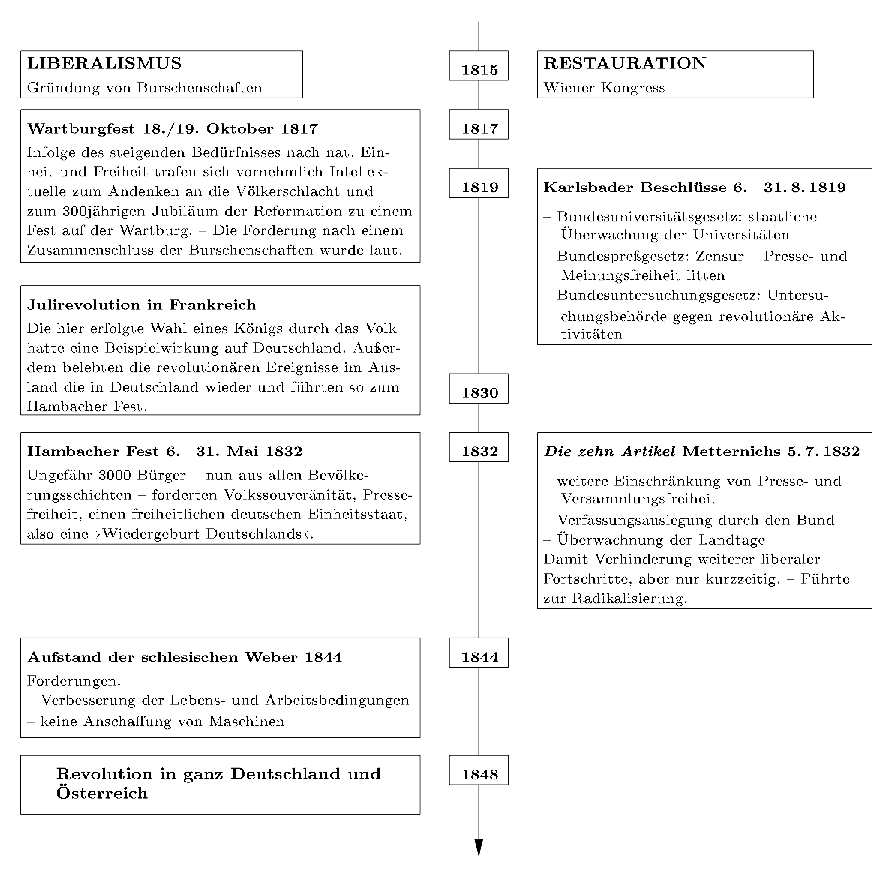
\includegraphics[width=\textwidth]{kampf-lib-rest.eps}
\caption{Das Ringen zwischen Liberalismus und Restauration}
\label{pic:kampf-lib-rest}
\end{figure}

Abbildung \ref{pic:kampf-lib-rest}\footnote{Die \ges{Zehn Artikel}
\Nam{Metternich, Klemens Wenzel Lothar von}{Metternichs} sind in
\cite{ZehnArt} zu finden, weitere Literatur in
\cite[106]{braunesGeschichts}. Die Quellen zu den übrigen Ereignissen
sind mir nicht bekannt.} zeigt die wichtigsten Ereignisse auf dem Weg
zur Revolution von 1848. Man erkennt, dass die Intensität von
antirestaurativen und restaurativen Maßnahmen immer weiter zunahm.
Weiter befeuert wurde die entwicklung durch die sich in Folge der
Industriellen Revolution verschärfenden soziale Lage.

%%%%%%%%%%%%%%%%%%%%%%%%%%%%%%%%%%%%%%%%%%%%%%%%%%%%%%%%%%%%%%%%%%%%%%

\subsection{Ursachenfeld}

\renewcommand*{\arraystretch}{1.5}
\newcolumntype{Y}{>{\setlength{\hsize}{0.55\hsize}\raggedleft}X}
\newcolumntype{Z}{>{\setlength{\hsize}{0.45\hsize}\raggedright}X}
\begin{tabularx}{\textwidth}{Y@{\quad$\lightning$\quad}Z}
restaurative Bewegung   & liberale Bewegung     \\
Absolutismus            & Aufklärung            \\
Industrielle Revolution -- Reichtum
                        & soziale Mißstände -- Armut    \\
territorialstaatlicher Absolutismus
                        & Einheitsbestrebungen
\end{tabularx}

%%%%%%%%%%%%%%%%%%%%%%%%%%%%%%%%%%%%%%%%%%%%%%%%%%%%%%%%%%%%%%%%%%%%%%

\subsection{Anlass}

Begünstigt durch die \dat{Krisenjahre 1847/48} in Frankreich mit
Missernten und Hungerunruhen kam es dort zur
\emph{Februarrevolution}\index{Februarrevolution}. Die Ereignisse in
Frankreich nahm man sich dann in Deutschland zum Vorbild und begann
die Revolution, die schon lange auf ihren Ausbruch gewartet hatte.
\mar{Germania und Bedeutung/Entwicklung von Symbolen.}

%%%%%%%%%%%%%%%%%%%%%%%%%%%%%%%%%%%%%%%%%%%%%%%%%%%%%%%%%%%%%%%%%%%%%%

\subsection{Verlauf}

\begin{figure}
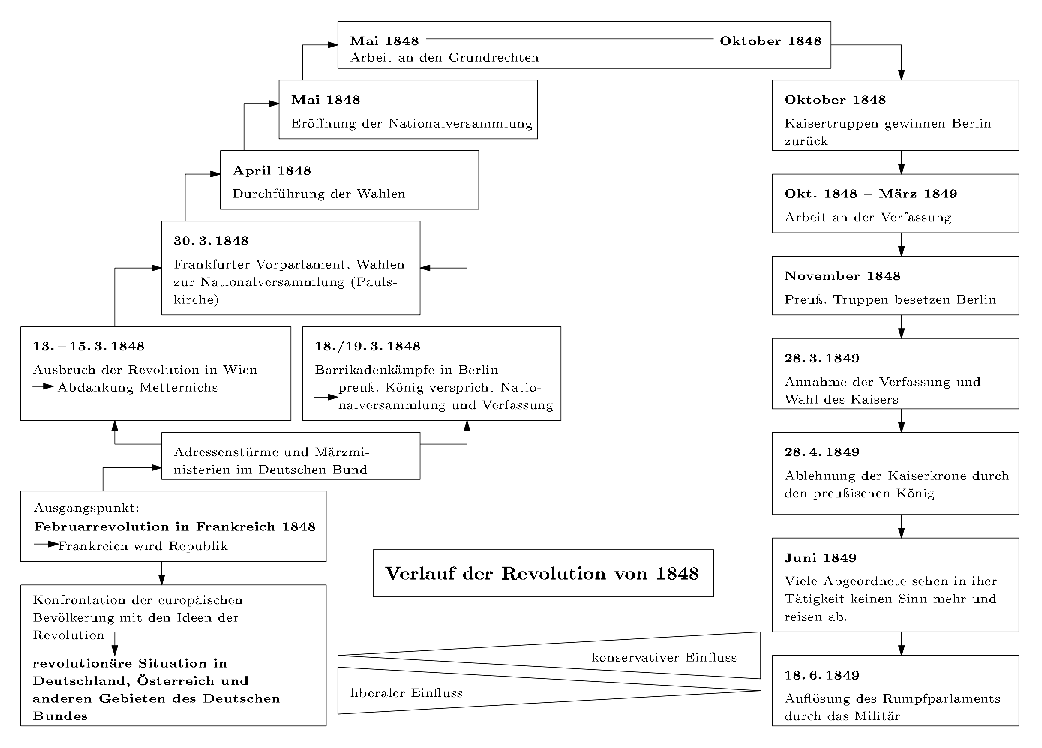
\includegraphics[height=\textwidth, angle=90]{verlauf-rev.eps}
\caption{Verlauf der Revolution von 1848}
\label{pic:verlauf-rev}
\end{figure}

Abbildung \ref{pic:verlauf-rev} bietet einen Überblick über den
Verlauf der Revolution. Diesen kann man in drei Etappen einteilen:
\mar{Richtige Benennung der Phasen?}

Die erste Phase war von kämpferischen Handlungen geprägt. Mit dem
Zusammentritt des \emph{Frankfurter Vorparlaments}
\index{Vorparlament!Frankfurt} begann eine Phase der Machtfestigung.
Der Niedergang setzte in der sehr langen Zeit der \emph{Arbeit an den
Grundrechten} ein. Diese Verzögerung der Vorgänge war nämlich einer
der Gründe für das Scheitern der Revolution: Durch die Uneinigkeit und
die fehlende parlamentarische Erfahrung, dauerte die Komprmissfindung
sehr lange. Das entstehende Machtvakuum nutzten die restaurativen
Kräfte für die Reaktion.

%%%%%%%%%%%%%%%%%%%%%%%%%%%%%%%%%%%%%%%%%%%%%%%%%%%%%%%%%%%%%%%%%%%%%%

\subsection{Verfassungsarbeit}

\begin{aufgabe}
Erläutern Sie die wesentlichen Aufgaben, die die
Paulskirchenversammlung zu lösen hatten und bilanzieren Sie die
jeweilige Lösung! 
\end{aufgabe}

\subsubsection{Parlament}

Das Parlament tagte in der runden
\Ort{Paulskirche!Frankfurt}{Frankfurter Paulskirche}\index{Frankfurt}.
Die 812 Männer unter dem Vorsitz des Liberalen \Nam{Gagern, Heinrich
von}{Heinrich von Gagern} waren hauptsächlich Bildungsbürger und
keinerlei Arbeiter. Man nannte die Versammlung daher auch
\jar{Parlament der Intellektuellen}.


\subsubsection{Grundrechte}
\index{Grundrechte}

Der erste Schwerpunkt der zukünftigten Verfassung für Deutschland
waren die Grundrechte. Auf Basis der Forderungen der Liberalen wurde
so ein umfangreicher Grundrechtskatalog beschlossen und im
\ort{Dezember 1848 angenommen}.


\subsubsection{Grenzen}

Eine sehr umstrittene Frage, die die Verhandlungen stark in die Länge
zog waren auch die zukünftigen Grenzen Deutschlands. Die
\emph{Großdeutsche Lösung} \index{Großdeutsche Lösung} sah neben den
deutschen Ländern die Einbeziehung der deutschsprachigen Teile
Österreichs vor. Diese wurde von vielen als die beste Variante
angesehen.

Österreich wollte jedoch sein gesamtes Staatsgebiet
einbringen, um als Gegengewicht zu Preußen auftreten zu können. Die
sogenannte \emph{Großösterreichische Lösung}
\index{Großösterreichische Lösung} war jedoch auch nicht möglich, da
man ein \emph{Deutsches} Reich wollte.

So fand man schließlich den Kompriss, Österreich ganz auszuschließen,
indem man zur \emph{Kleindeutschen Lösung} \index{Kleindeutschen
Lösung} gelangte.


\subsubsection{Staat}

Auch der \emph{Staatsaufbau} war Gegenstand langer Diskussionen zwischen
Demokraten, die eine Republik wollten und Liberalen, die eine
konstitutionelle Monarchie befürworteten. Das Ergebnis war das
System, welches Abbildung \ref{pic:verf-paulsk}\mar{Scan aus braunem
Geschichtsbuch S. 128 einfügen.} zeigt. \mar{Kriterien für
Verfassungsbewertung: Machtballungen, Rolle des Volkes, Verhältnis der
Organe} Es fallen dabei besonders die weitgreifenden Befugnisse des
Kaisers, die nicht mit dem Prinzip der Gewaltenteilung zu vereinbaren
sind, die freien Gerichte und der ausgeprägte Föderalismus auf.

Das Paulskirchenparlament musste auch die Entscheidung über das
künftige \emph{Staatsoberhaupt} fällen. Man wählte den Preußenkönig
\nam{Friedrich Wilhelm \Rm{4}}. Dieser lehnte allerdings ab, da er die
Krone nur \jar{aus den Händen eines deutschen Fürsten} empfangen
wollte. Die Verfassung war damit gescheitert.

%%%%%%%%%%%%%%%%%%%%%%%%%%%%%%%%%%%%%%%%%%%%%%%%%%%%%%%%%%%%%%%%%%%%%%

\mar{Das nennt sich wohl Bilanz.}
\subsection{Leistungen und Grenzen}

\begin{aufgabe}
Erörtern Sie die Darstellung, indem Sie die Hauptaussagen zur Wertung
der Revolution herausarbeiten, begründen, warum die Revolution trotz
iher fortschrittlichen Ideen scheiterte und sich zum Begriff des
epochalen Einschnitts für das Jahr 1848 positionieren!
\end{aufgabe}

\mar{?}
\begin{itemize}
\item Wertung der Verfassung
\item Nachweis des fraktionellen Kompromisses 
\end{itemize}

\subsubsection[Gründe des Scheiterns]{Gründe des
Scheiterns\mycite[138\,--\,140]{braunesGeschichts}}

\begin{itemize}
\item keine Hauptstadt $\rightarrow$ Polyzentrismus (viele kleine
Revolutionsherde)
\item keine parlamentarischen Machtmittel (Geld, Truppen)
\item Furcht vor Weiterführung der Revolution in soziale Revolution
\item Macht der Einzelmonarchen
\item Uneinigkeit durch unterschiedliche Ziele (auch sozial)
\item Unterschätzung der konservativen Kräfte
\end{itemize}


\subsubsection[Bedeutung für die deutsche Geschichte]{Bedeutung für
die deutsche Geschichte\mycite[140/141]{braunesGeschichts}}

\begin{itemize}
\item zuerst starke Zurückdrängung der liberalen Bewegung
\item Bestehenbleiben des Verfassungsstaates (konstitutionelle
Monarchien) in den deutschen Ländern außer Österreich
\item Abschaffung der Zensur

\item keine weitere Infragestellung von
\begin{itemize}
\item Bauernbefreiung
\item Ende der adeligen Patrimonialgerichtsbarkeit
\item Ende der Sonderrechte des Adels
\end{itemize}

\item moderne Gewerbeordnung
\item Obrigkeit sieht Reformbedürftigkeit ein
\item neues politisches Bewusstsein -- \emph{Geburtsstunde der Parteien}
\index{Parteien!Geburtsstunde}
\item Verfassungs- und Grundrechtsidee
\end{itemize}

%%%%%%%%%%%%%%%%%%%%%%%%%%%%%%%%%%%%%%%%%%%%%%%%%%%%%%%%%%%%%%%%%%%%%%

\subsection{Von der \jar{Revolution von unten} zur \jar{Revolution von
oben}}
\index{Revolution!von unten}
\index{Revolution!von oben}

Bereits \dat{Ende 1848} oktroyierte \nam{Friedrich Wilhelm \Rm{4}} in
Preußen eine Verfassung und kam damit den liberalen Bestrebungen in
geringem Maße selbst nach, setzte aber auch eindeutig seine Politik
durch. -- Sie enthielt unter anderem folgende Bestimmungen:

\begin{itemize}
\item Pressefreiheit
\item Gleichheit vor dem Gesetz
\item Zweikammersystem -- \Ins{Herrenhaus!Preußen}{Herrenhaus} vom
König berufen, \Ins{Abgeordnetenhaus!Preußen}{Abgeordnetenhaus} von
der Bevölkerung gewählt
\item Dreiklassenwahlrecht \index{Dreiklassenwahlrecht!Preußen} bei
öffentlicher und indirekter Wahl
\item Gesetze bedürfen der Zustimmung beider Häuser
\end{itemize}

Im Gegensatz zu Preußen hob Österreich \dat{1851 seine Verfassung
wieder auf} und kehrte damit zum Absolutismus zurück.

Schon \dat{1850} vereinbarten beide Staaten die \dat{Wiederherstellung
des \Ins{Deutscher Bund}{Deutschen Bundes}}. Mit der
\dat{Wiedereröffnung des \Ins{Frankfurter Bundestages}{Frankfurter
Bundestages} am 12. Mai 1851} und mit der \dat{Aufhebung der
\ges{Grundrechte des deutschen Volkes} im August} hatte in Preußen die
Reaktion endgültig gesiegt.

Folgende zwei Auszüge spiegeln das Klima der damaligen Zeit wider: Das
erste aus dem ausklingenden Vormärz mit deutlich appellativem
Charakter, das zweite aus der anbrechenden Zeit des Biedermeier
\index{Biedermeier} zeugt von Resignation\footnote{Liest man den
vollständigen Text, offenbart sich ein etwas anderer Charakter, doch
im Unterricht wurde wieder einmal auf die Praktik der Verheimlichung
zurückgegriffen.}:

\poemtitle*{Männer aus dem Proletariat!\mycite{ProlMaen} (1848)}
\settowidth{\versewidth}{geprügelt und geplagt von den erbärmlichsten
Gendarmentröpfen,}

\begin{verse}[\versewidth]
Handwerksburschen, \\
die ihr am Bettelstabe Deutschland durchzieht, \\
geschunden von den jammervollsten Polizeischergen, \\
geprügelt und geplagt von den erbärmlichsten Gendarmentröpfen, \\
laßt Euch doch nicht länger mehr als Hunde behandeln, \\
steht auf, fletscht die Zähne \mbox{[\dots]}! 
\end{verse}

\poemtitle*{\Nam{Pfau, Ludwig}{Ludwig Pfau} (1821\,--\,1891):
Badisches Wiegenlied (1849)\mycite{PfauWiegenl}}
\settowidth{\versewidth}{Und wer nicht schläft in guter Ruh’,}

\begin{verse}[\versewidth]
Schlaf’, mein Kind, schlaf leis’, \\
Dort draußen geht der Preuß’, \\
Deinen Vater hat er umgebracht, \\
Deine Mutter hat er arm gemacht, \\
Und wer nicht schläft in guter Ruh’, \\
Dem drückt der Preuß’ die Augen zu. \\
Schlaf’, mein Kind, schlaf leis’, \\
Dort draußen geht der Preuß’, \\!

Schlaf’, mein Kind, schlaf leis’, \\
Dort draußen geht der Preuß’, \\
Der Preuß' hat eine blut’ge Hand, \\
Die streckt er über’s badische Land, \\
Und alle müssen stille sein \\
Als wie dein Vater unterm Stein \\
Schlaf’, mein Kind, schlaf leis’, \\
Dort draußen geht der Preuß’,  \\
\mbox{[\dots]} \\
\end{verse}

%%%%%%%%%%%%%%%%%%%%%%%%%%%%%%%%%%%%%%%%%%%%%%%%%%%%%%%%%%%%%%%%%%%%%%

\subsection{Bilanz der liberalen Bewegung}

\begin{itemize}
\item \emph{Altliberale} galten als Verlierer der Revolution und
bildeten weiter den Gegenpol zur konservativen Bewegung.

\item Durch Industrialisierung gestärktes Wirtschaftsbürgertum
(\emph{Bourgeoisie}\index{Bourgeoisie}) suchte nach Kompromissen mit
den Konservativen (\emph{Realpolitiker}\index{Realpolitiker}).

\item Die Regentschaft des preußischen Kronprinzen seit \dat{1858} und
seit 1861 Köngis \Nam{Wilhelm \Rm{1}} begründete eine \dat{\beg{Neue
Ära}} in Preußen.
\end{itemize}

Das neue Kabinett brachte allerdings eine Reihe von Problemen mit
sich: Das \ins{Herrenhaus}, welches vom Junkeradel \index{Junkeradel}
dominiert wurde, blockierte nämlich von nun an alle Neuerungen. So kam
es dann auch zu dem Konflikt zwischen Konservativen und Liberalen um
eine Heeresreform (Aufstockung), der sich zu einem Verfassungskonflikt
auswuchs. Die Liberalen der zweiten Kammer bewilligten nämlich nur
einen provisorischen Haushalt für \dat{1860/1861}, woraufhin die
Konservativen reagierten, indem sie das Mitspracherecht des Parlaments
in Militärangelegenheiten einschränkten und so das Budgetrecht
aushebelten. Infolgedessen spalteten sich die Linksliberalen von den
Altliberalen ab und gründeten zusammen mit den Demokraten \dat{1861
die \ins{Fortschrittspartei}}, die erste klassische Partei auf
deutschem Boden.

\endinput




\endinput
